\section{Results}

In this section, we compare the results from Moltres for each benchmark step to
the results reported in the the benchmark paper \citep{tiberga_results_2020}.
The benchmark paper contains results from four different \gls{MSR} simulation
software packages. The software packages from \textit{CNRS} and \textit{TUD}
each report two sets of results arising from different angular discretizations
in their neutronics software. These are designated as \textit{CNRS-SP$_1$} and
\textit{CNRS-SP$_3$}; and \textit{TUD-S$_2$} and \textit{TUD-S$_6$},
respectively. The authors of the benchmark performed code-to-code
verification by reporting the average discrepancy $\epsilon$ of each observable
along the centerlines AA' and/or BB' from each software for each
benchmark step. The discrepancy $\epsilon_c$ from each software package for
each measured observable $Q_c$ calculated using the following equation:
%
\begin{align}
    \epsilon_c &= \sqrt{\frac{\sum^{N_p}_{i=1}\left(Q_c(\vec{r_i}) - Q_{avg}
    (\vec{r_i})\right)^2}{\sum^{N_p}_{i=1} Q^2_{avg}(\vec{r_i})}}
    \intertext{where}
    N_p &= 201 \nonumber \\
    &= \mbox{number of sampling points of quantity $Q$,}
    \nonumber \\
    N_c &= \mbox{number of \gls{MSR} software packages,} \nonumber \\
    Q_{avg}(\vec{r_i}) &= \frac{1}{N_c} \sum^{N_c}_{c=1} Q_c(\vec{r_i})
    \nonumber \\
    &= \mbox{average value of $Q$ at $\vec{r_i}$ from all packages.} \nonumber
\end{align}

For observables measured along the centerlines AA' and/or BB', this section
reports the average percentage discrepancy of each observable from Moltres in
Tables \ref{table:disc0} and \ref{table:disc1} alongside the overall average
percentage discrepancy of all software
packages involved in the \textit{CNRS benchmark}.
%In addition, this section
%also includes tables of point-wise observable values at nine equidistant points
%along the centerlines to facilitate the results discussion and a direct
%comparison to the same data provided by \cite{tiberga_results_2020} in their
%\textit{CNRS benchmark} paper.
We also reproduced similar plots from the
benchmark paper for every observable along AA'
or BB' in Figures \ref{fig:0.1}, \ref{fig:0.2}, \ref{fig:0.3}, \ref{fig:1.1},
\ref{fig:1.2}, \ref{fig:1.3}, and \ref{fig:2.1} for a qualitative
comparison of the results from Moltres and the benchmark. All reactivity and
change in reactivity results from Steps 0.2, 1.1, 1.2, and
1.3 are collated into Table \ref{table:rho}.

\subsection{Phase 0 results \& discussion}
%
\begin{figure}[h!]
	\centering
    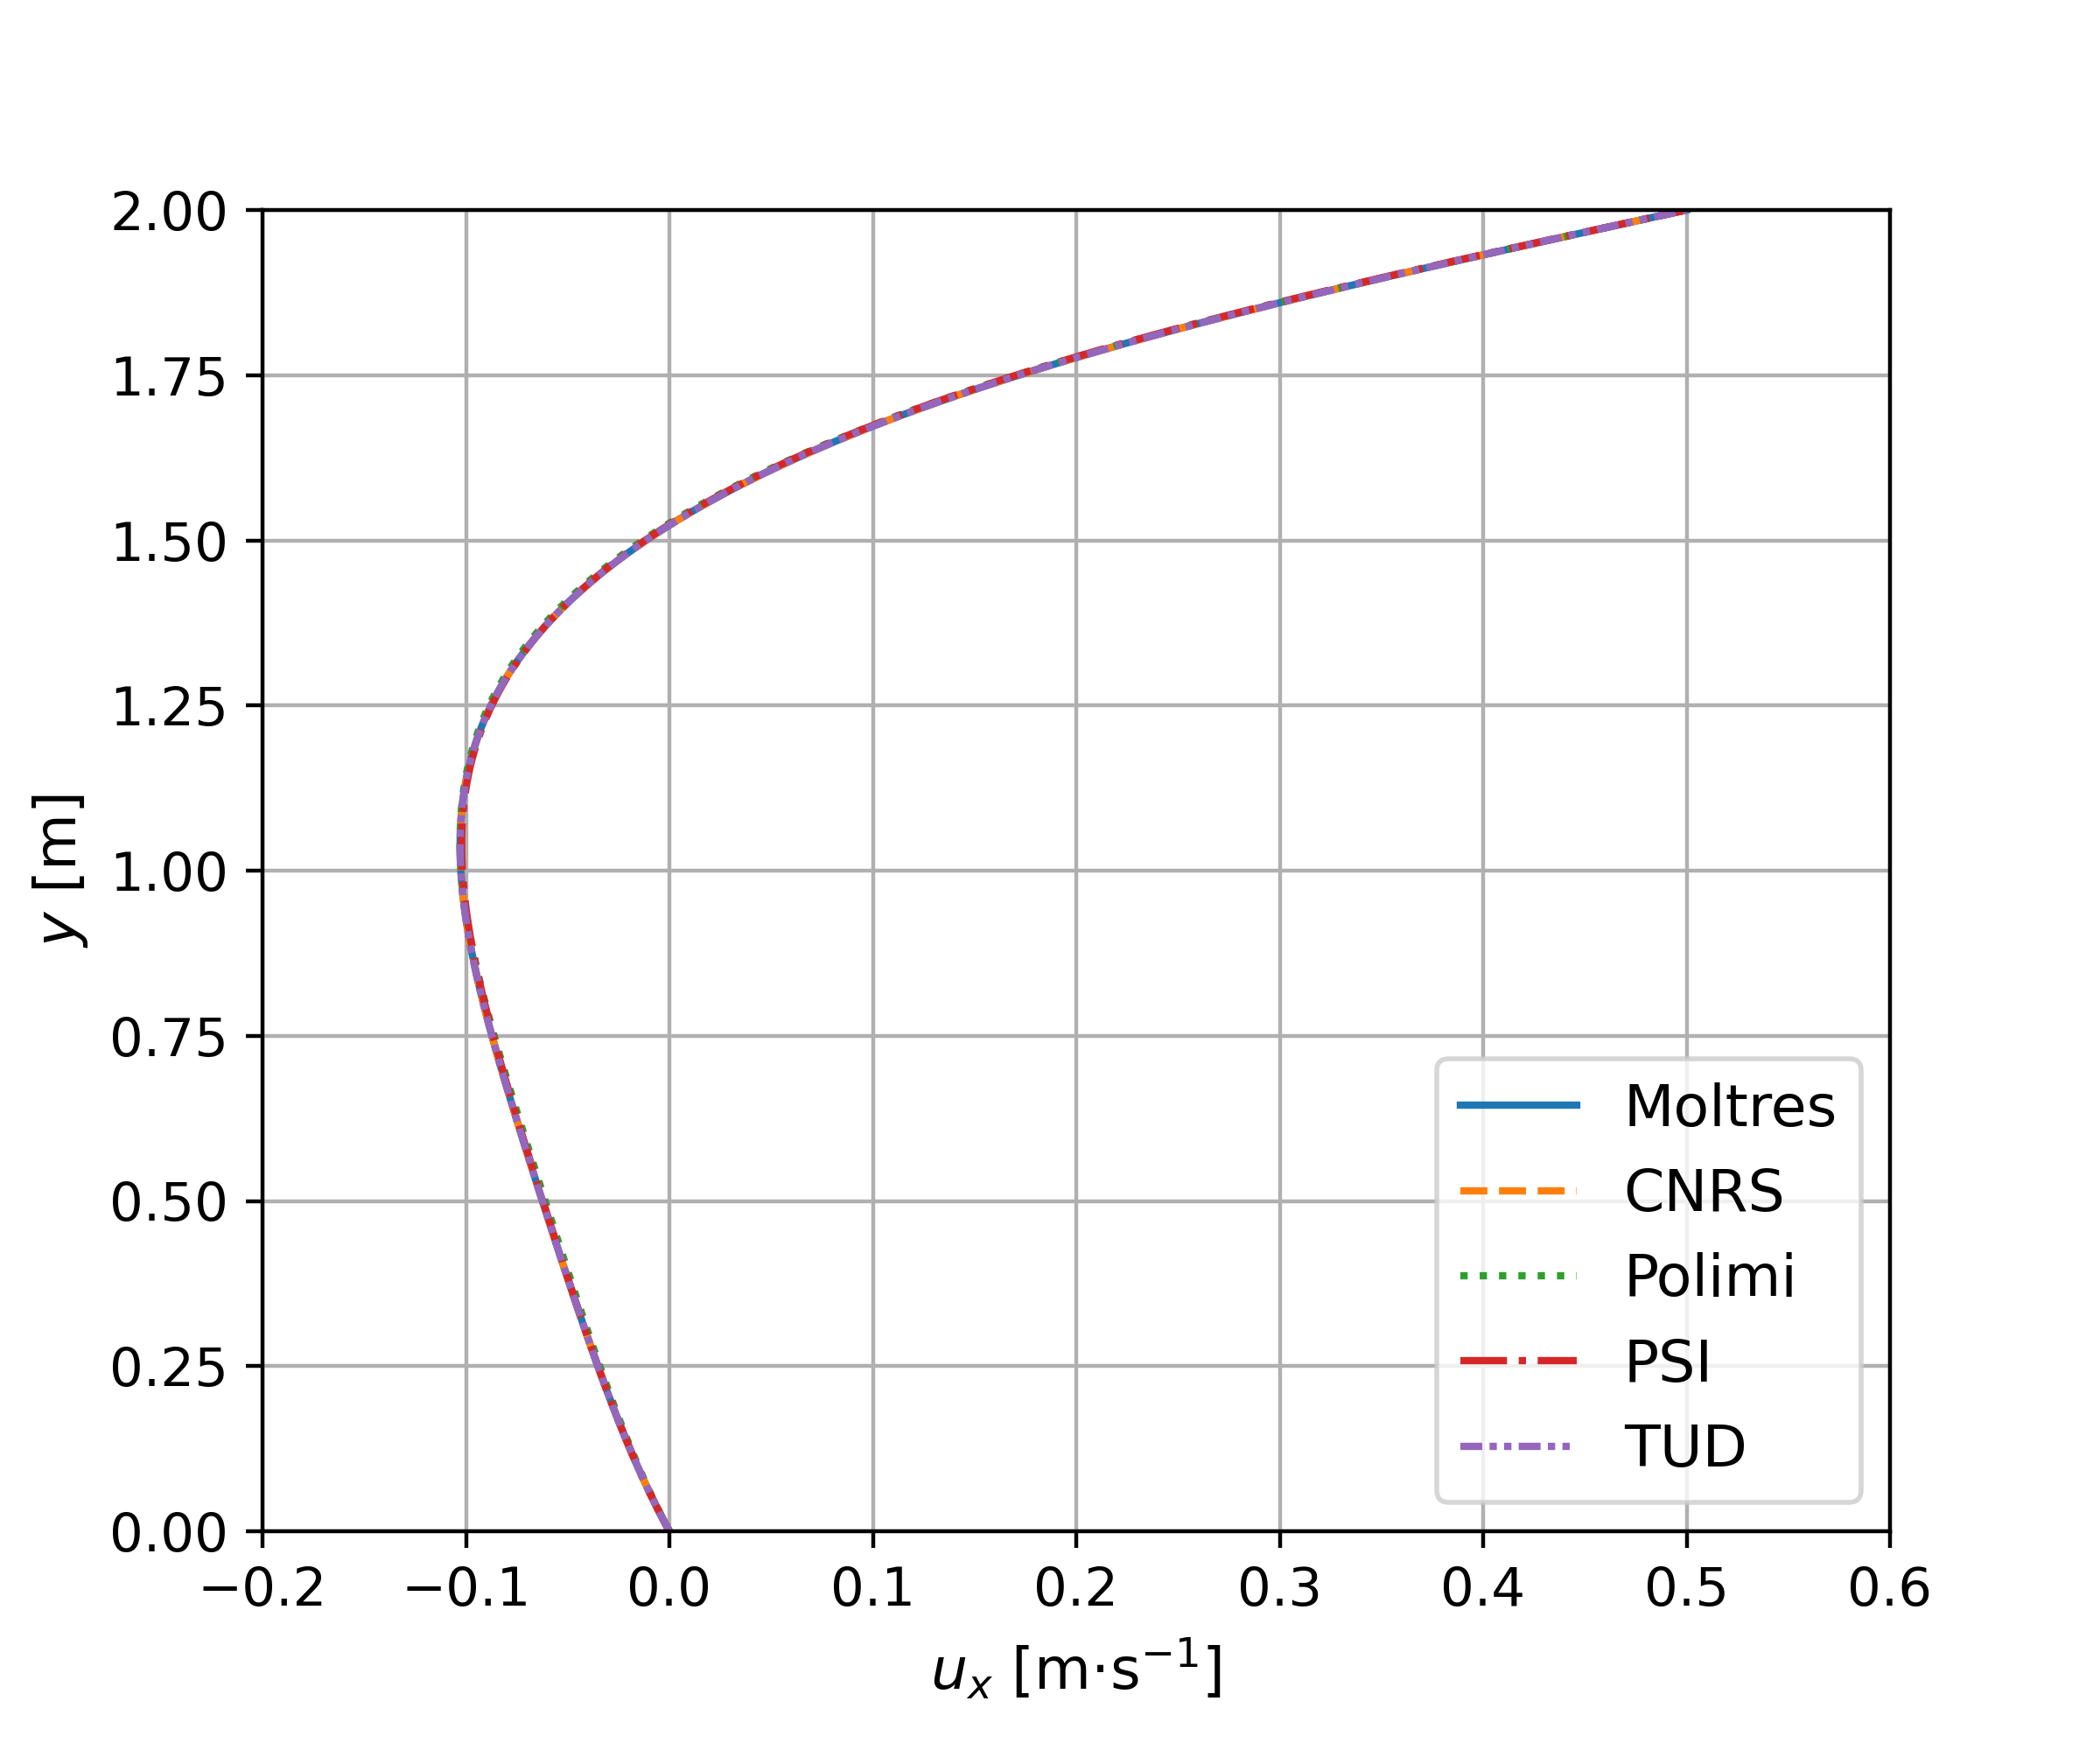
\includegraphics[width=.8\columnwidth]{0-1-vel-plot}
	\caption{Step 0.1 - Horizontal velocity component along BB'.}
	\label{fig:0.1}
\end{figure}
%
\begin{figure}[h!]
	\centering
	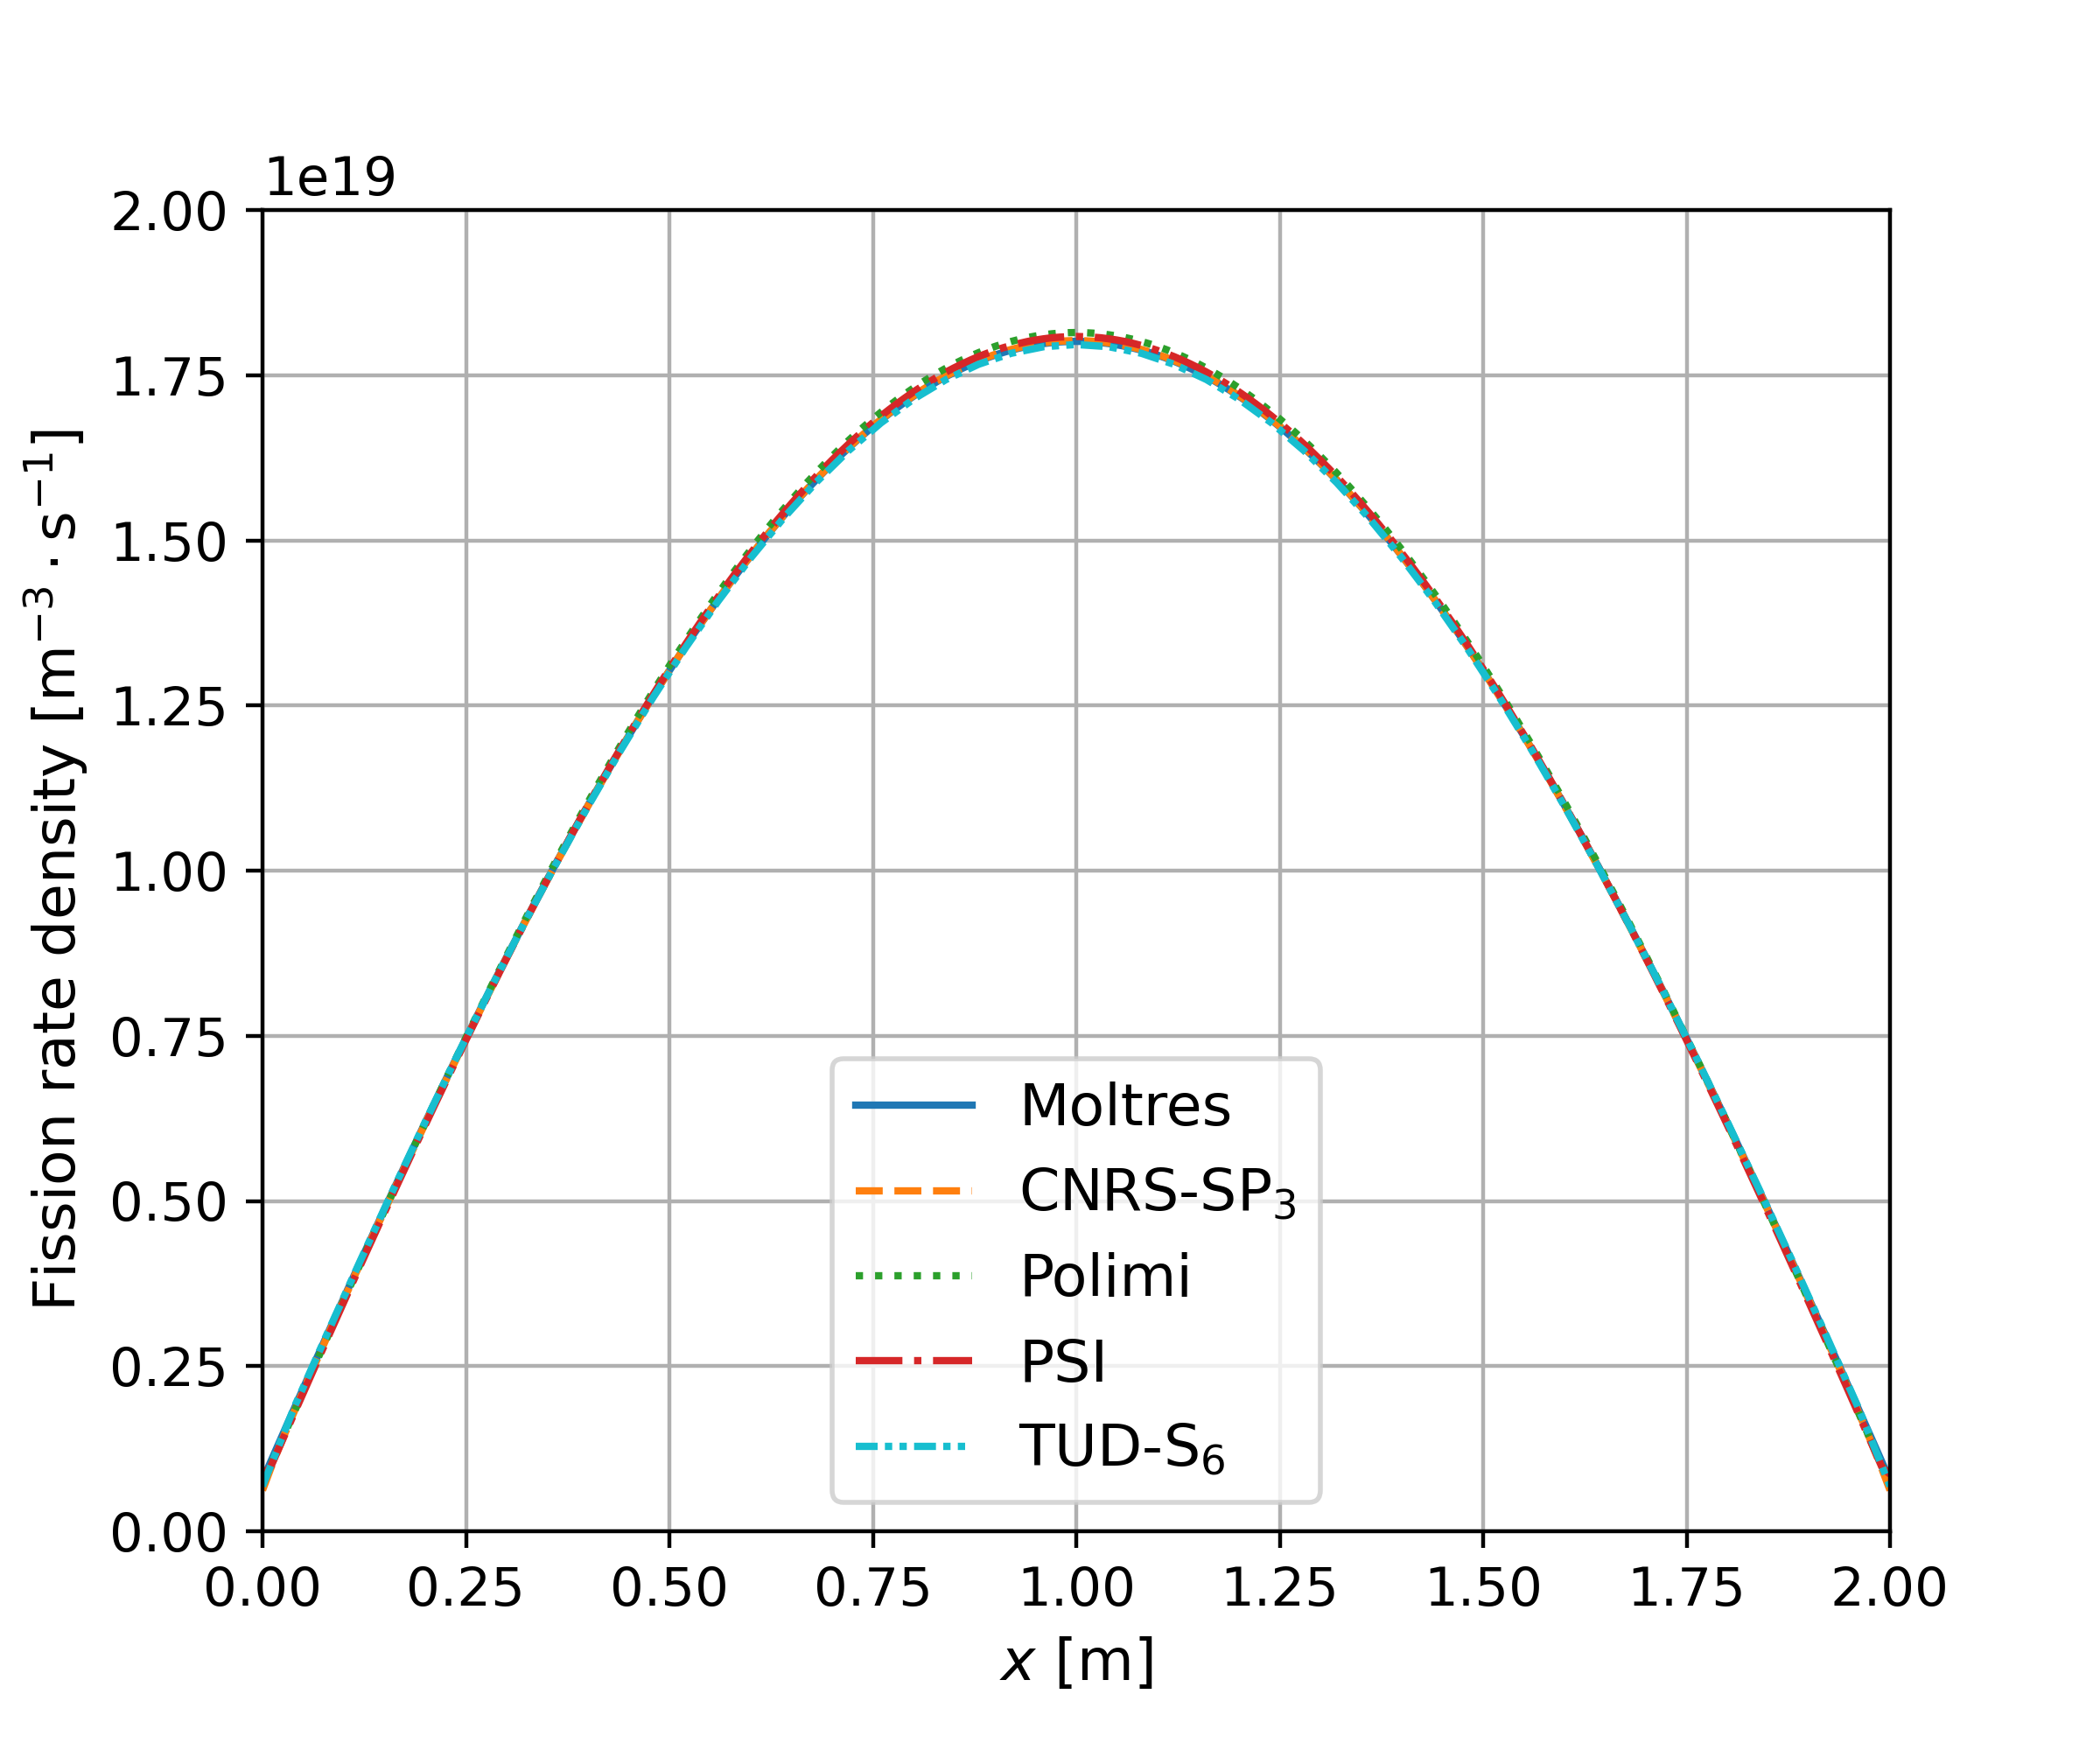
\includegraphics[width=.8\columnwidth]{0-2-fiss-plot}
	\caption{Step 0.2 - Fission rate density along AA'.}
	\label{fig:0.2}
\end{figure}
%
\begin{figure}[h!]
	\centering
	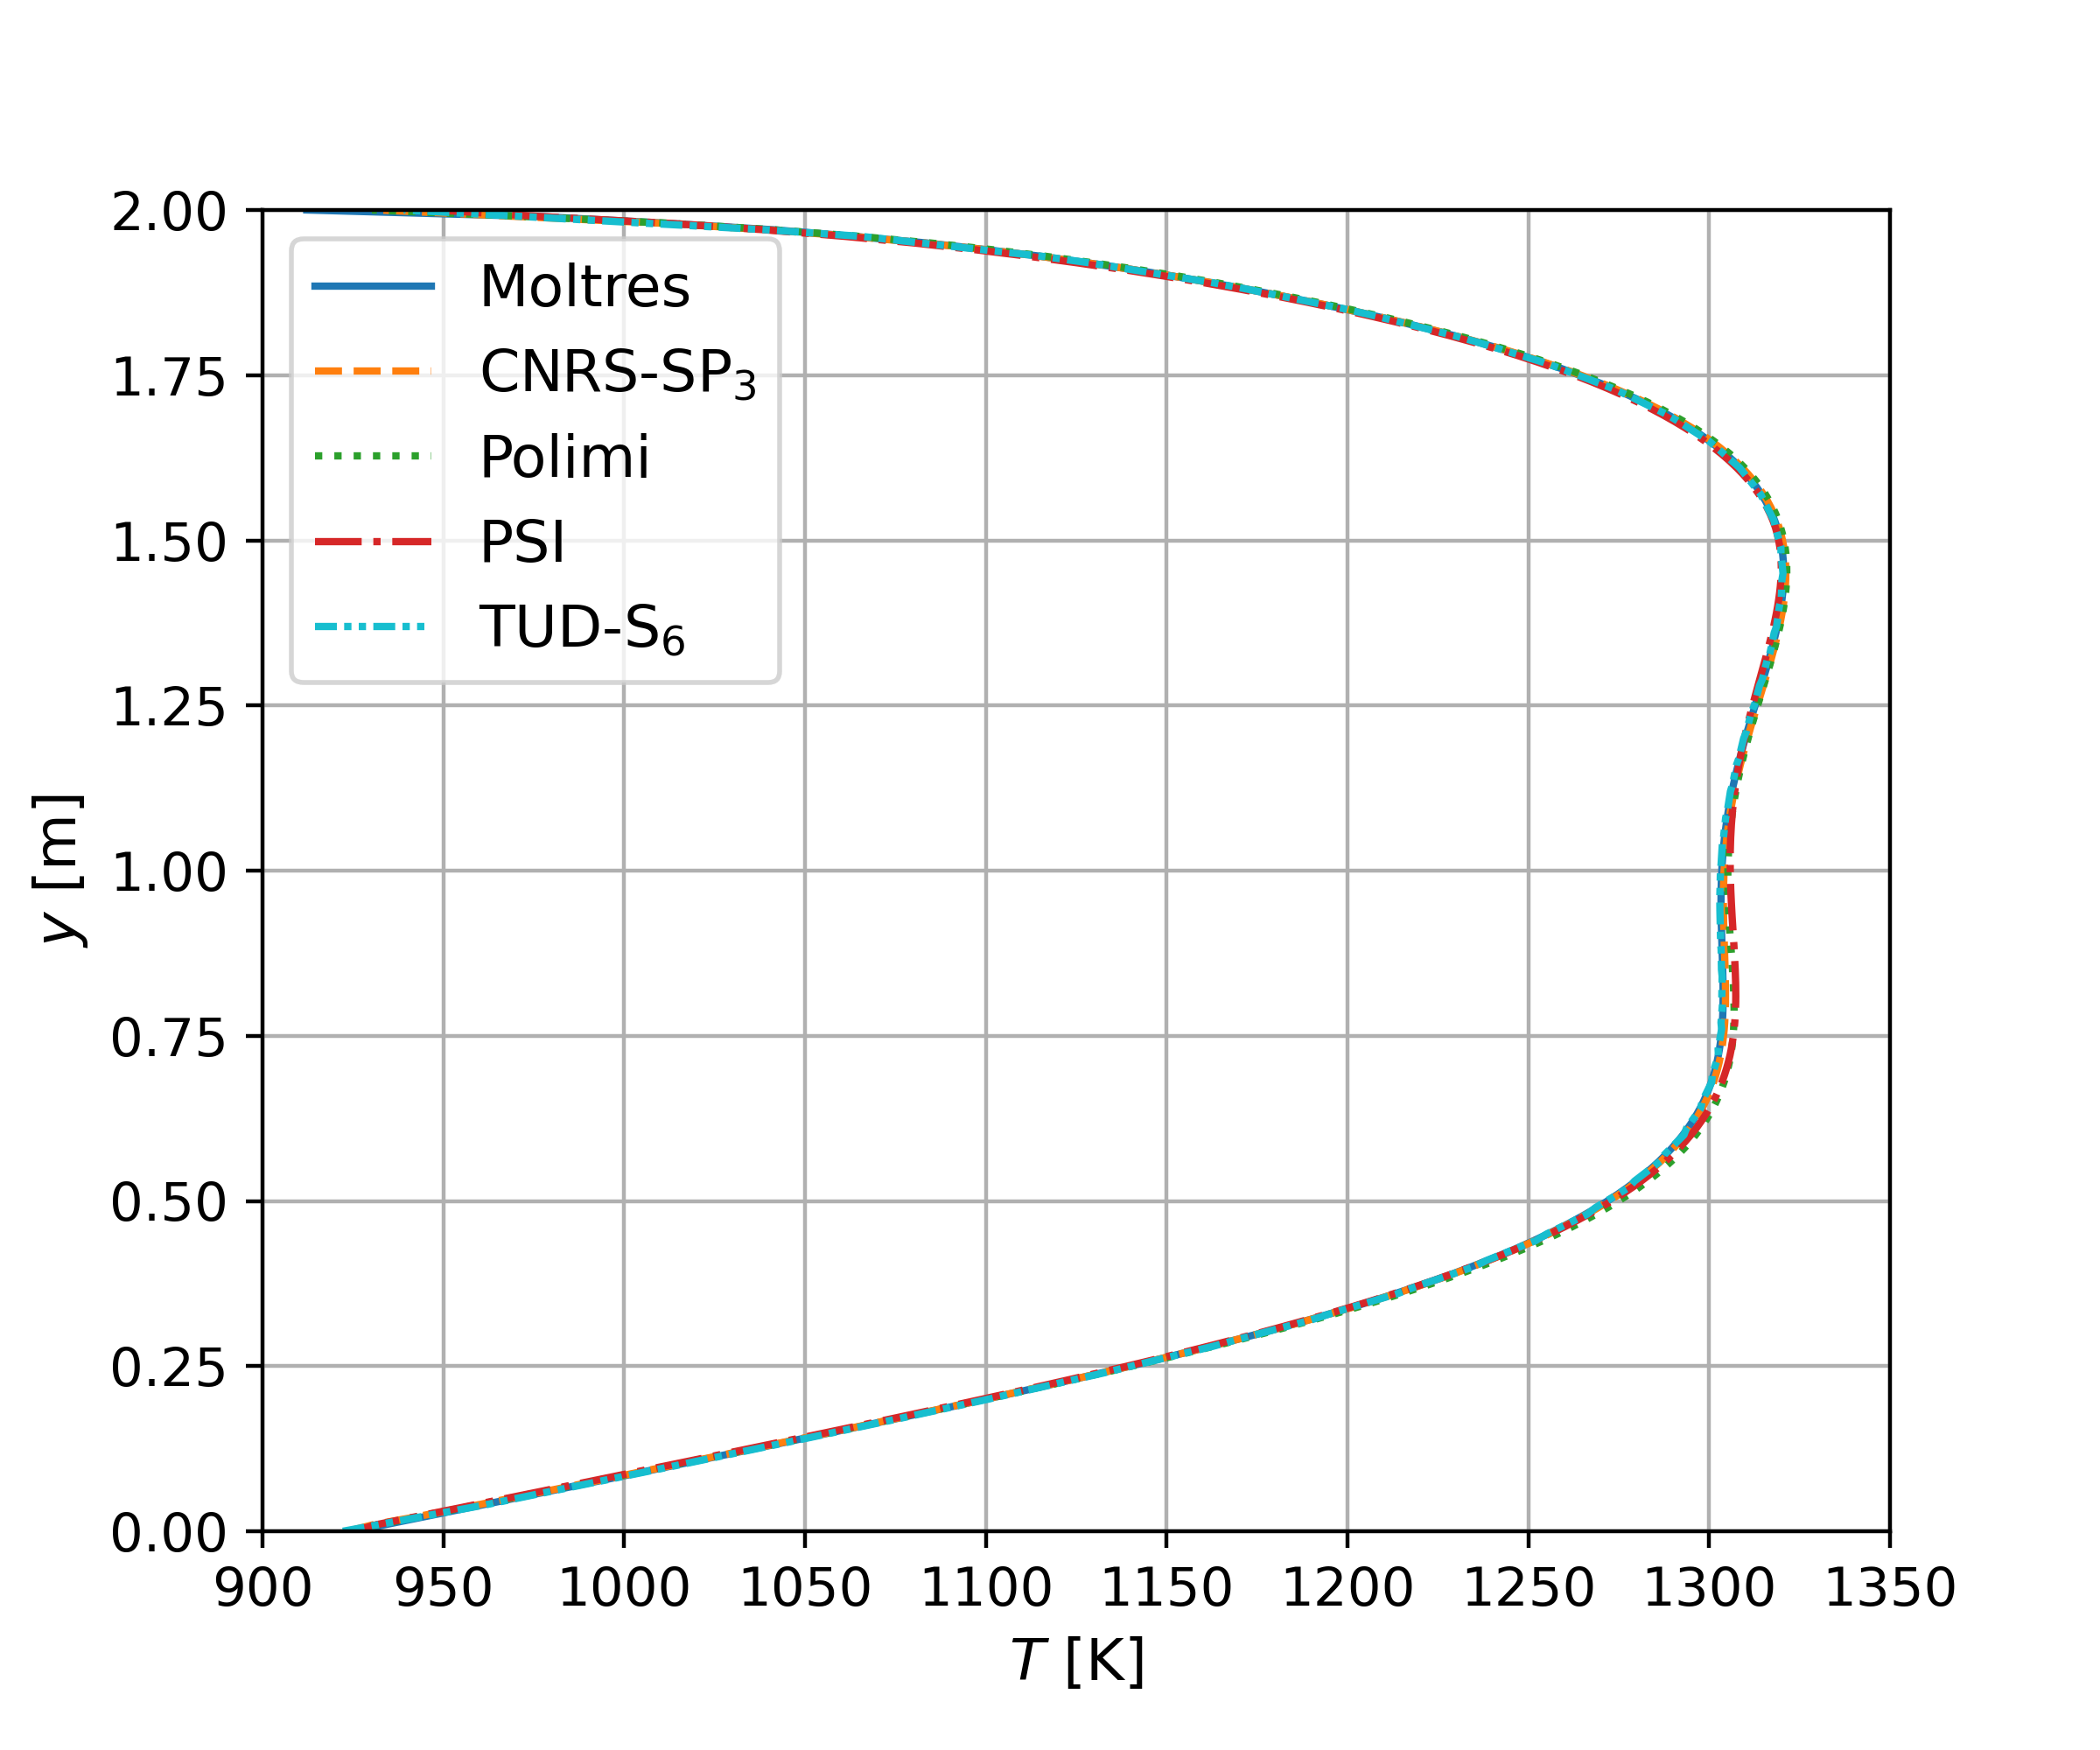
\includegraphics[width=.8\columnwidth]{0-3-temp-plot}
	\caption{Step 0.3 - Temperature distribution along BB'.}
	\label{fig:0.3}
\end{figure}

Figures \ref{fig:0.1}, \ref{fig:0.2}, and \ref{fig:0.3} show that Moltres
accurately reproduced all three sets of results in Phase 0 for the velocity
field, fission rate density, and temperature, respectively.
Table \ref{table:disc0} reports the discrepancy values from Moltres for Phase 0
and the corresponding average discrepancy values from the benchmark
\citep{tiberga_results_2020}. Moltres performs excellently as all discrepancy
values are on the same order of magnitude as those from the benchmark,
except the discrepancy value for $T$ along centerline BB' which is marginally
higher at 0.164\% compared to 0.083\% from the benchmark average. However, we
note in Figure \ref{fig:0.3} that the $T$ distribution from Moltres shows good
agreement with the corresponding distributions from the CNRS-$SP_3$ and
TUD-$S_6$ results.
%This
%exception is a natural consequence of having the $T$ distribution calculations
%in Step 0.3 depend on the velocity field and neutron flux from the previous 
%Steps; the $T$ distributions, as shown in Figure \ref{fig:0.3}, show visibly
%less overlap (around $y=0.75$ m) compared to the $u_x$ and fission rate density
%distributions in Figures \ref{fig:0.1} and \ref{fig:0.2}, respectively.

Table \ref{table:temp} shows the temperature values from Moltres and the
benchmark at nine equidistant points along centerlines AA' and BB'. Unlike the
general trend seen in Figure \ref{fig:0.3}, the
temperature value for Moltres at the end of centerline BB', on the top
boundary, deviated significantly (912 K from Moltres
vs. ~935 K from the benchmark) because this point along the top boundary is
directly downstream of the discontinuous velocity boundary condition on the
top-left corner of the domain. Without the SUPG and PSPG stabilization schemes,
the singularity would produce spurious oscillations which extended well into
the interior region of the domain. 

Finite element methods struggles with
the velocity boundary condition discontinuity on the top left corner of the
domain. As such, we observe the temperature deviation
directly downstream of the discontinuity. However, we note that all other
temperature values agree closely with the benchmark data. 

We also observe in table \ref{table:rho} that the reactivity $\rho$ value of
465.6 pcm from Moltres falls well within the range of $\rho$ values from the
benchmark. Moltres' $rho$ value agrees closest to the results from the software
packages which adopted the neutron diffusion and theoretical-equivalent models,
namely the CNRS-$SP_1$, Polimi, PSI, and TUD-$S_2$ software.

\begin{table}[h!]
	\caption{Discrepancy values for the results from Phase 0.}
	\centering
	\footnotesize
	\begin{tabular}{l l c S S}
		\toprule
		\multirow{2}{*}{\textbf{Step}} & \multirow{2}{*}{\textbf{Observable}} & \multirow{2}{*}{\textbf{Centerline}} & \multicolumn{2}{c}{\textbf{Discrepancies [\%]}} \\
		& & & {Moltres} & {Benchmark} \\
		\midrule
		\multirow{4}{*}{0.1} &
		\multirow{2}{*}{$u_x$ [m$\cdot$s$^{-1}$]} & AA' & 0.247 & 0.253 \\
		& & BB' & 0.266 & 0.318 \\
		\cmidrule{2-5}
		& \multirow{2}{*}{$u_y$ [m$\cdot$s$^{-1}$]} & AA' & 0.540 & 0.598
		\\
		& & BB' & 0.468 & 0.795 \\
		\midrule
		{0.2} &
		{$\sum^G_i \Sigma_{f,i} \phi_i(\vec{r})$
		[m$^{-3}\cdot$s$^{-1}$]} & AA' & 0.313 & 0.285 \\
		\midrule
		\multirow{2}{*}{0.3} &
		\multirow{2}{*}{$T$ [K]} & AA' & 0.090 & 0.085 \\
		& & BB' & 0.164 & 0.083 \\
		\bottomrule
	\end{tabular}
	\label{table:disc0}
\end{table}
%
\begin{table*}[htb!]
	\caption{Temperature distribution along centerlines $AA'$ and $BB'$.}
	\centering
	\footnotesize
	\setlength\tabcolsep{1.5pt}
	\begin{tabular}{c c c c c c c c c c c}
		\toprule
		\multirow{2}{*}{\textbf{Observable}} & \multirow{2}{*}{\textbf{Code}} & \multicolumn{9}{c}{\textbf{Results along $AA'$} (point coordinates are expressed in m)} \\
		& & {(0,1)} & {(0.25,1)} & {(0.5,1)} & {(0.75,1)} & {(1,1)} & {(1.25,1)} & {(1.5,1)} & {(1.75,1)} & {(2,1)} \\
		\midrule
		\multirow{7}{*}{$T$ (K)} & Moltres & 9.251E+02 & 1.194E+03 & 1.357E+03 & 1.361E+03 &
		1.303E+03 & 1.224E+03 & 1.131E+03 & 1.035E+03 & 9.251E+02 \\
		& CNRS-$SP_1$ & 9.253E+02 & 1.194E+03 & 1.358E+03 & 1.363E+03 & 1.305E+03 & 1.224E+03 & 1.131E+03 & 1.034E+03 & 9.251E+02 \\
		& CNRS-$SP_3$ & 9.236E+02 & 1.194E+03 & 1.357E+03 & 1.361E+03 & 1.304E+03 & 1.224E+03 & 1.131E+03 & 1.034E+03 & 9.235E+02 \\
		& Polimi & 9.253E+02 & 1.196E+03 & 1.361E+03 & 1.364E+03 & 1.305E+03 & 1.224E+03 & 1.132E+03 & 1.035E+03 & 9.252E+02 \\
		& PSI & 9.253E+02 & 1.196E+03 & 1.356E+03 & 1.363E+03 & 1.306E+03 & 1.226E+03 & 1.133E+03 & 1.037E+03 & 9.252E+02 \\
		& TUD-$S_2$ & 9.212E+02 & 1.194E+03 & 1.359E+03 & 1.364E+03 & 1.305E+03 & 1.224E+03 & 1.131E+03 & 1.032E+03 & 9.225E+02 \\
		& TUD-$S_6$ & 9.219E+02 & 1.194E+03 & 1.356E+03 & 1.360E+03 & 1.303E+03 & 1.223E+03 & 1.131E+03 & 1.034E+03 & 9.233E+02 \\
		\midrule
		\midrule
		\multirow{2}{*}{\textbf{Observable}} & \multirow{2}{*}{\textbf{Code}} & \multicolumn{9}{c}{\textbf{Results along $BB'$} (point coordinates are expressed in m)} \\
		& & {(1,0)} & {(1,0.25)} & {(1,0.5)} & {(1,0.75)} & {(1,1)} & {(1,1.25)} & {(1,1.5)} & {(1,1.75)} & {(1,2)} \\
		\midrule
		\multirow{7}{*}{$T$ (K)} & Moltres & 9.251E+02 & 1.140E+03 & 1.272E+03 & 1.303E+03 &
		1.303E+03 & 1.313E+03 & 1.320E+03 & 1.264E+03 & 9.123E+02 \\
		& CNRS-$SP_1$ & 9.252E+02 & 1.139E+03 & 1.273E+03 & 1.305E+03 & 1.305E+03 & 1.314E+03 & 1.321E+03 & 1.265E+03 & 9.322E+02 \\
		& CNRS-$SP_3$ & 9.236E+02 & 1.140E+03 & 1.272E+03 & 1.304E+03 & 1.304E+03 & 1.313E+03 & 1.320E+03 & 1.265E+03 & 9.322E+02 \\
		& Polimi & 9.253E+02 & 1.140E+03 & 1.275E+03 & 1.307E+03 & 1.305E+03 & 1.313E+03 & 1.321E+03 & 1.265E+03 & 9.303E+02 \\
		& PSI & 9.252E+02 & 1.139E+03 & 1.273E+03 & 1.307E+03 & 1.306E+03 & 1.312E+03 & 1.319E+03 & 1.263E+03 & 9.481E+02 \\
		& TUD-$S_2$ & 9.215E+02 & 1.139E+03 & 1.273E+03 & 1.305E+03 & 1.305E+03 & 1.315E+03 & 1.322E+03 & 1.265E+03 & 9.374E+02 \\
		& TUD-$S_6$ & 9.222E+02 & 1.140E+03 & 1.272E+03 & 1.303E+03 & 1.303E+03 & 1.312E+03 & 1.319E+03 & 1.264E+03 & 9.390E+02 \\
		\bottomrule
	\end{tabular}
	\label{table:temp}
\end{table*}
%
\begin{table}[h!]
    \caption{Reactivity $\rho$ and change in reactivity
    $\left(\rho_a - \rho_b\right)$ values from Steps 0.2, 1.1,
    1.2, and 1.3. All units are in pcm.}
    \centering
    \footnotesize
    \begin{tabular}{l S S S S}
        \toprule
        \multirow{2}{*}{\textbf{Software}} & {\textbf{Step 0.2}} &
        {\textbf{Step 1.1}} & {\textbf{Step 1.2}} & {\textbf{Step 1.3}} \\
        & {$\rho_{s_{0.2}}$}
        & {$\rho_{s_{1.1}} - \rho_{s_{0.2}}$}
        & {$\rho_{s_{1.2}} - \rho_{s_{1.1}}$}
        & {$\rho_{s_{1.3}} - \rho_{s_{0.2}}$} \\
        \midrule
        Moltres     & 465.6 & -62.7 & -1142.2 & -1207.7 \\
        CNRS-$SP_1$ & 411.3 & -62.5 & -1152.0 & -1220.5 \\
        CNRS-$SP_3$ & 353.7 & -62.6 & -1152.7 & -1220.7 \\
        Polimi      & 421.2 & -62.0 & -1161.0 & -1227.0 \\
        PSI         & 411.7 & -63.0 & -1154.8 & -1219.6 \\
        TUD-$S_2$   & 482.6 & -62.0 & -1145.2 & -1208.5 \\
        TUD-$S_6$   & 578.1 & -60.7 & -1122.0 & -1184.4 \\
        \bottomrule
    \end{tabular}
    \label{table:rho}
\end{table}

\subsection{Phase 1 results \& discussion}

Figure \ref{fig:color} shows the typical temperature distribution and velocity
streamlines from running a fully coupled problem in Step 1.4. 
Table \ref{table:disc1} shows the discrepancy values from Moltres for Steps
1.1, 1.2, and 1.3,
and the corresponding average discrepancy values from the benchmark
\citep{tiberga_results_2020}. The subsequent subsections discuss the results
for each benchmark step.
%
\begin{figure}[h!]
  \centering
  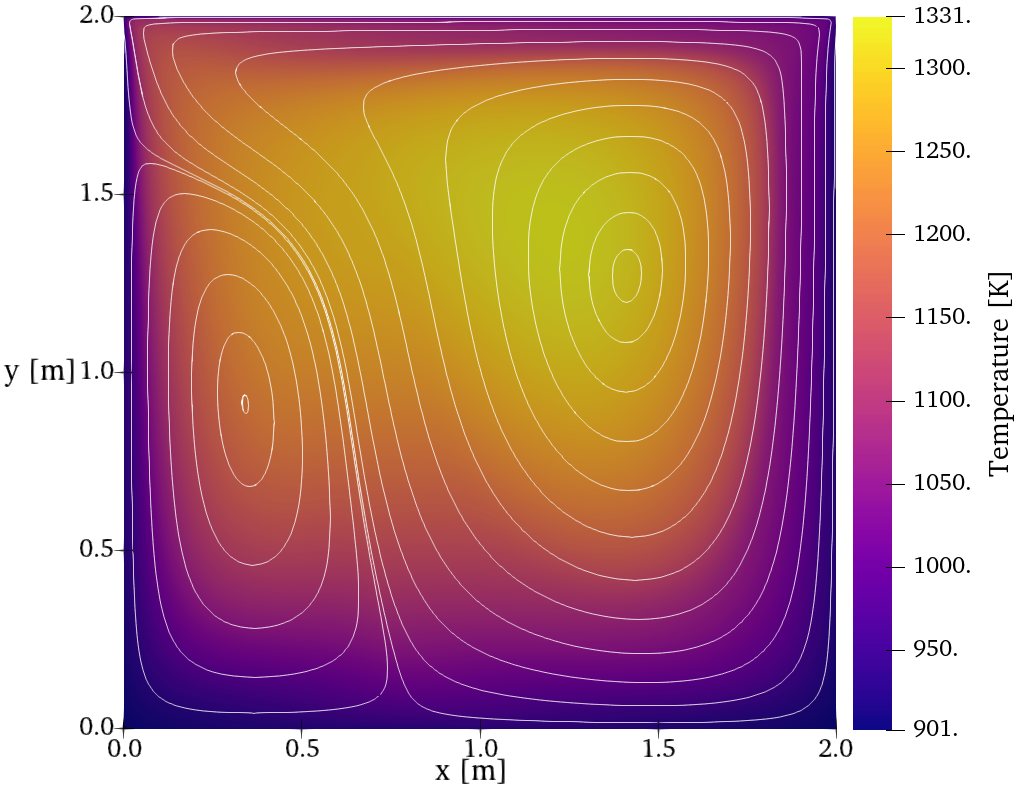
\includegraphics[width=\columnwidth]{full-coupled}
  \caption{The temperature distribution in the domain for the fully coupled
  system (Step 1.4) with buoyancy effects, $P = 1$ GW, and $U_{lid} = 0.5$
  m$\cdot$s$^{-1}$. The lines correspond to the streamlines of the velocity
  field.}
  \label{fig:color}
\end{figure}

\subsubsection{Step 1.1: Circulating fuel}

Moltres performs relatively worse than the benchmark average, but the
discrepancies are still on the same order of magnitude. We attribute this to
the same zeroth-order shape function approximation for the precursor
concentration mentioned in Step 0.2.

On the other hand, we observe in Table \ref{table:rho} that the change in
$\rho$ relative to Step 0.2 falls within the reported range of $\rho$ values
from the benchmark.

%
\begin{figure}[h!]
	\centering
    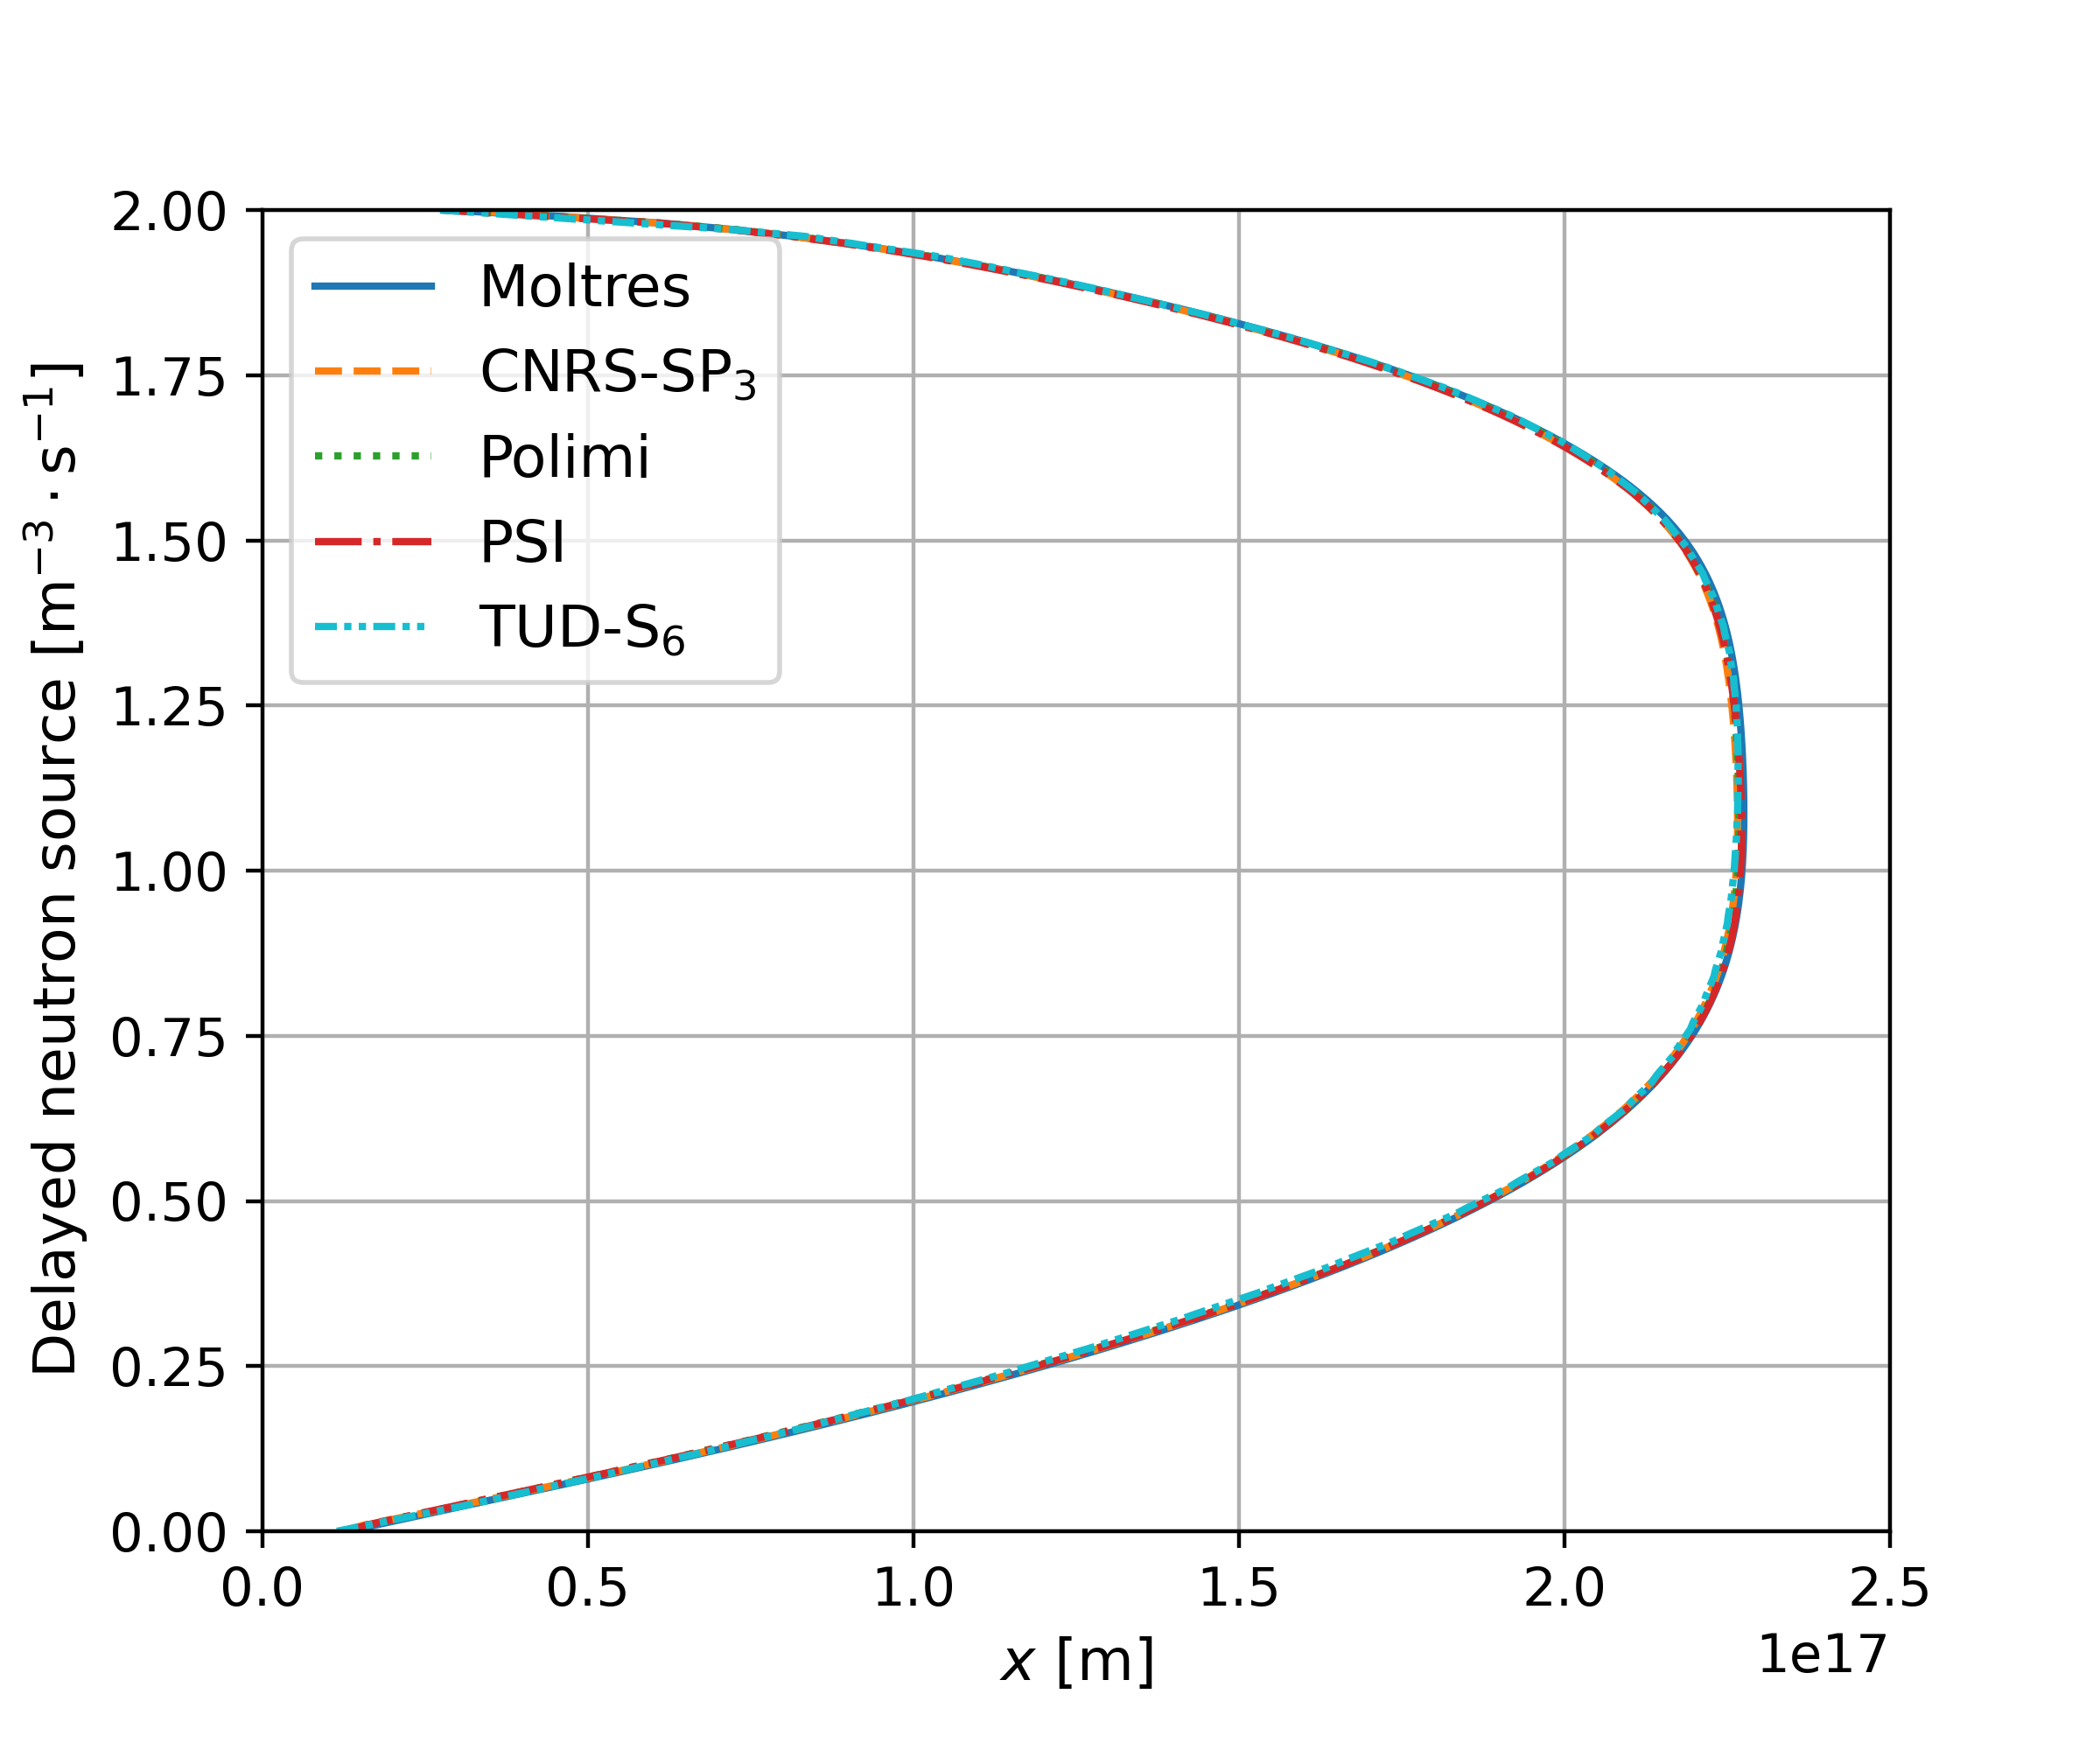
\includegraphics[width=.8\columnwidth]{1-1-dnp-plot}
	\caption{Step 1.1 - Delayed neutron source along BB'.}
	\label{fig:1.1}
\end{figure}
%
\begin{table*}[htb!]
	\caption{Discrepancy values for the results from Phase 1.}
	\centering
	\footnotesize
	\begin{tabular}{l l c S S}
		\toprule
		\multirow{2}{*}{\textbf{Step}} & \multirow{2}{*}{\textbf{Observable}} & \multirow{2}{*}{\textbf{Centerline}} & \multicolumn{2}{c}{\textbf{Discrepancies [\%]}} \\
		& & & {Moltres} & {Benchmark} \\
		\midrule
		\multirow{2}{*}{1.1} &
		\multirow{2}{*}{$\sum_j \lambda_j C_j$ [m$^{-3}\cdot$s$^{-1}$]} & AA' & 0.603 & 0.346 \\
		& & BB' & 0.327 & 0.294 \\
		\midrule
		\multirow{4}{*}{1.2} &
		\multirow{2}{*}{$T$ [K]} & AA' & 0.076 & 0.095 \\
		& & BB' & 0.179 & 0.089 \\
		\cmidrule{2-5}
		& \multirow{2}{*}{\footnotesize $\Delta\left[\sum^G_i \Sigma_{f,i} \phi_i(\vec{r})
		\right]_{s_{1.2}-s_{0.2}}$ [m$^{-3}\cdot$s$^{-1}$]} & AA' & 1.110 & 1.576 \\
		& & BB' & 1.082 & 1.133 \\
		\midrule
		\multirow{7}{*}{1.3} &
		{$u_x$ [m$\cdot$s$^{-1}$]} & AA' & 0.123 & 0.691 \\
		\cmidrule{2-5}
		& \multirow{2}{*}{$u_y$ [m$\cdot$s$^{-1}$]} & AA' & 0.237 & 0.329 \\
		& & BB' & 0.238 & 0.356 \\
		\cmidrule{2-5}
		& \multirow{2}{*}{$T$ [K]} & AA' & 0.064 & 0.057 \\
		& & BB' & 0.070 & 0.080 \\
		\cmidrule{2-5}
		& \multirow{2}{*}{$\sum_j \lambda_j C_j$ [m$^{-3}\cdot$s$^{-1}$]} & AA' & 1.043 & 0.460 \\
		& & BB' & 0.462 & 1.194 \\
		\bottomrule
	\end{tabular}
	\label{table:disc1}
\end{table*}

\subsubsection{Step 1.2: Power coupling}

For this step, Moltres performed better than the benchmark average except
the temperature distribution along BB', the cause of which we
addressed in Step 0.3. The smaller discrepancy in the change in fission rate
density indicates that Moltres is on average more self-consistent since this
quantity measures the difference between two sets of data from the same
software. From Table \ref{table:rho}, Moltres also reports a change in $\rho$,
relative to Step 1.1, that falls within the range of benchmark values.
%
\begin{figure*}[h!]
	\centering
	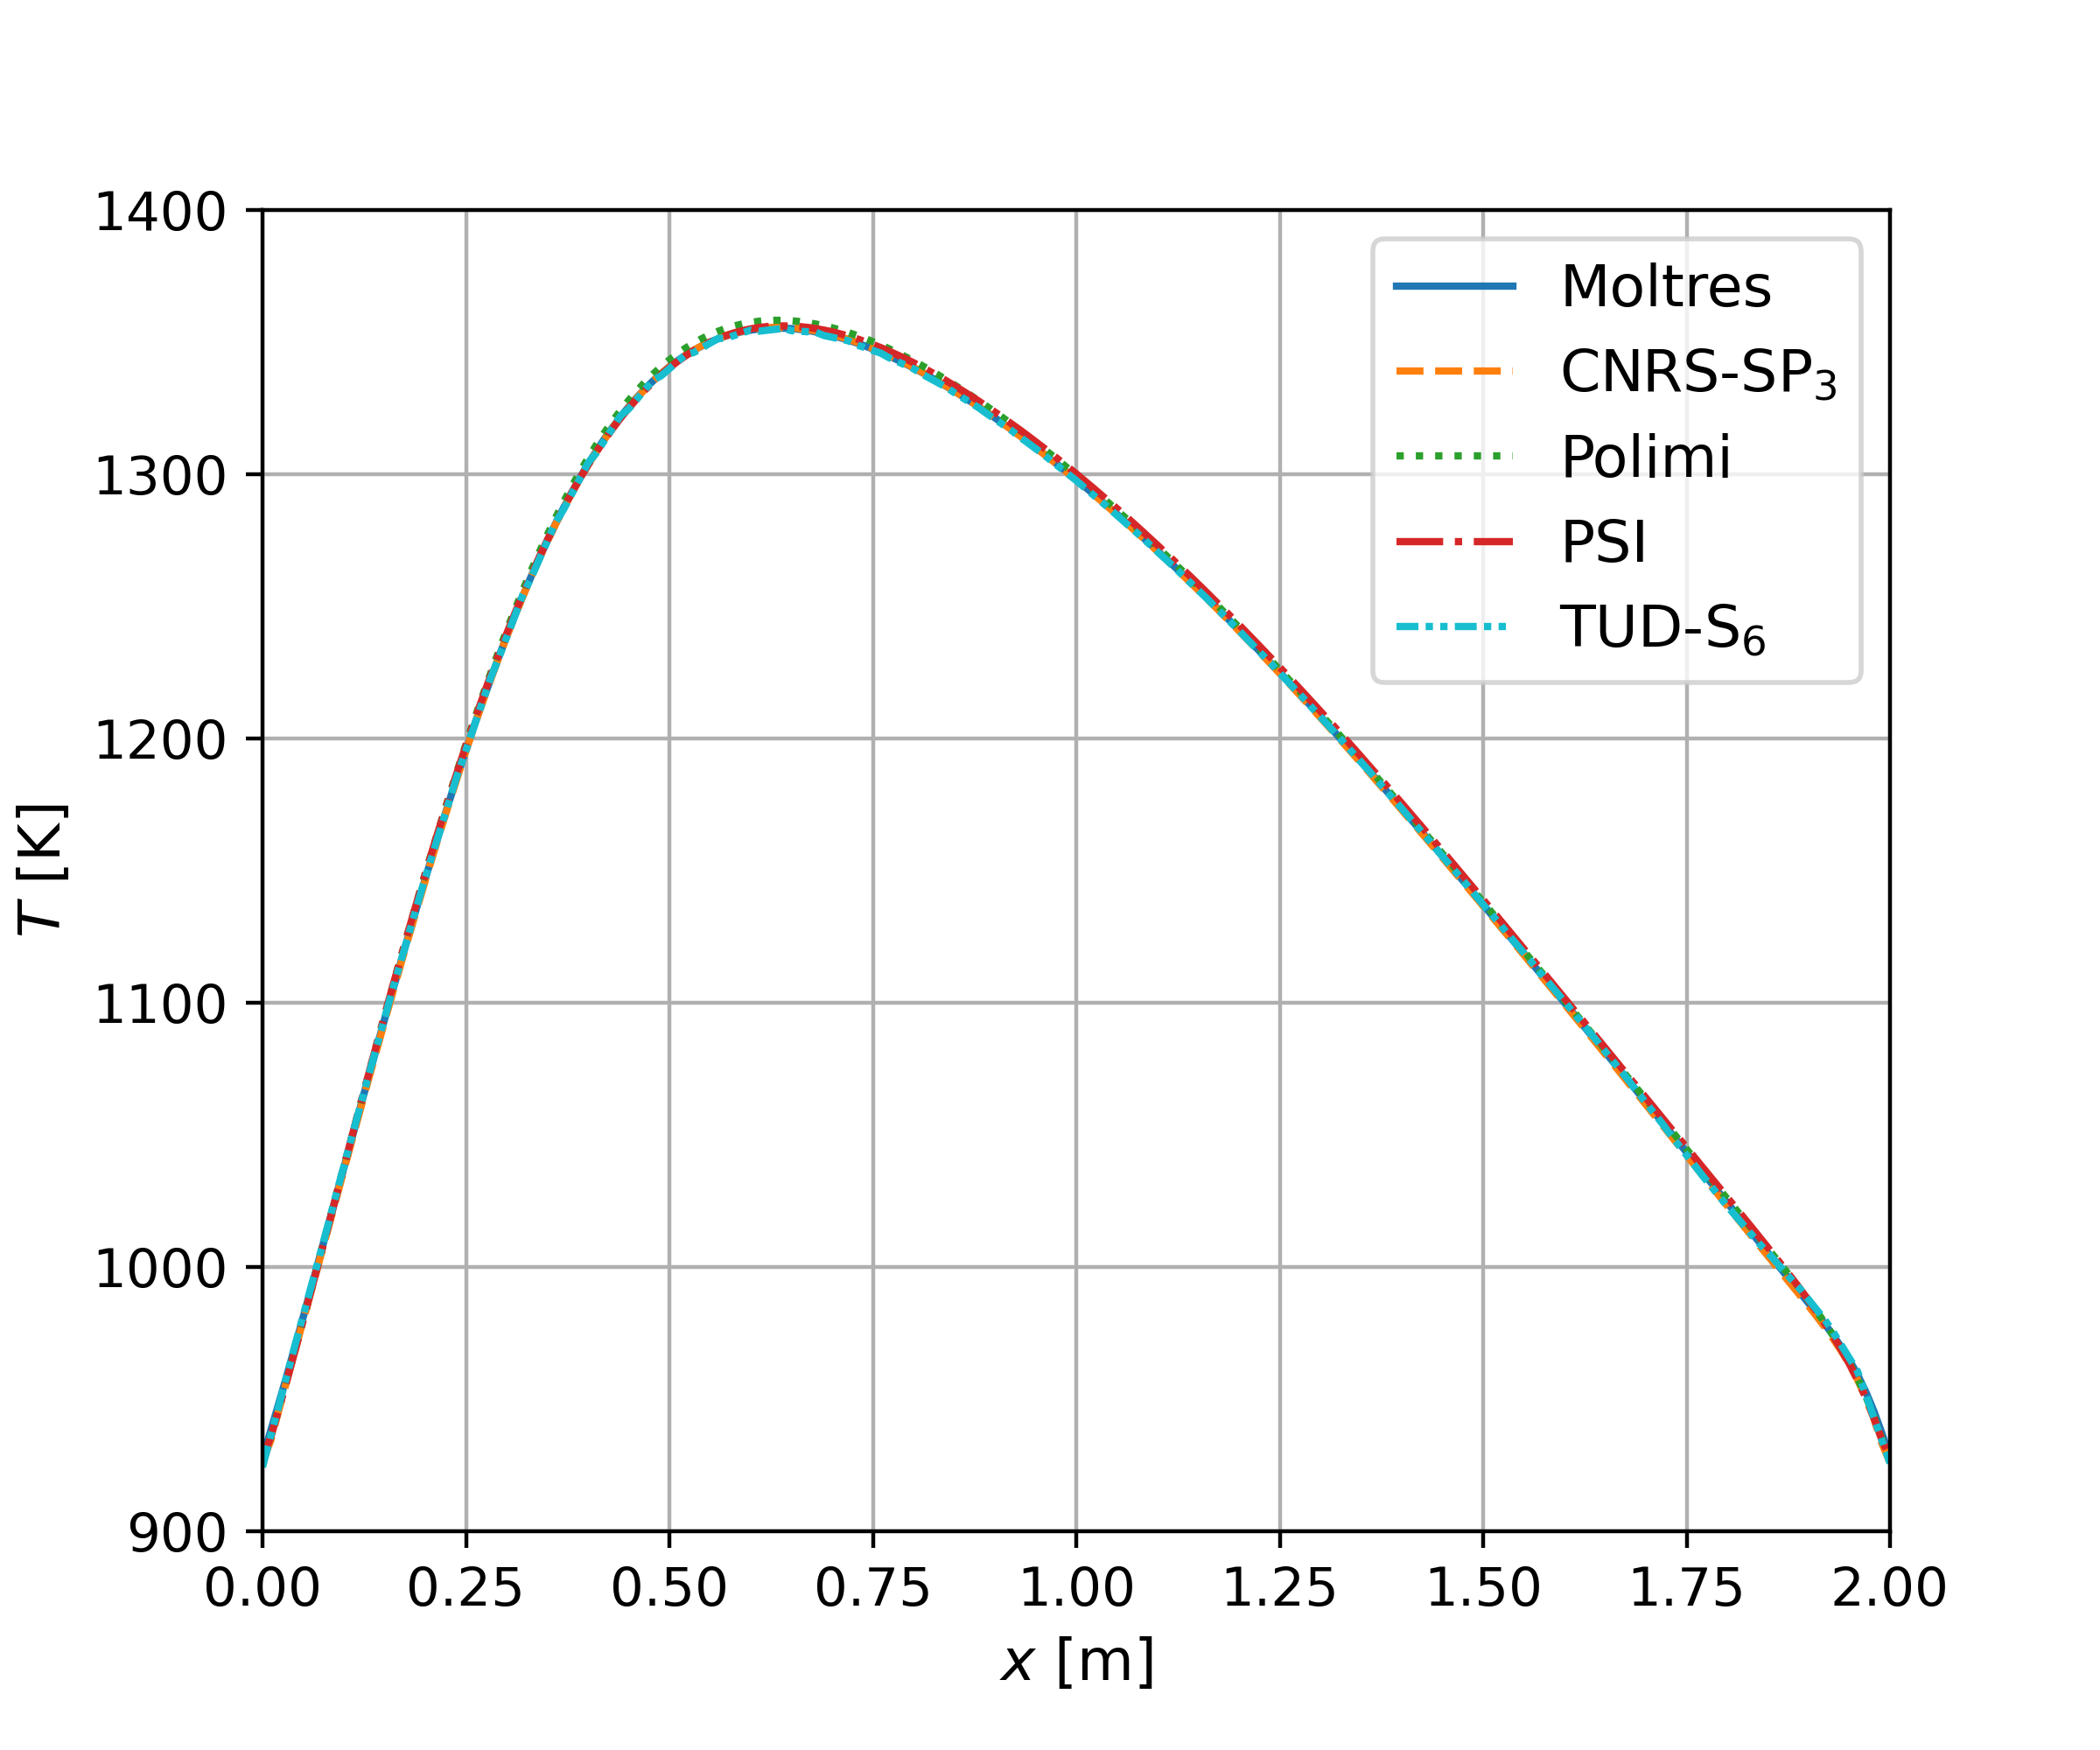
\includegraphics[width=.8\columnwidth]{1-2-temp-plot}
	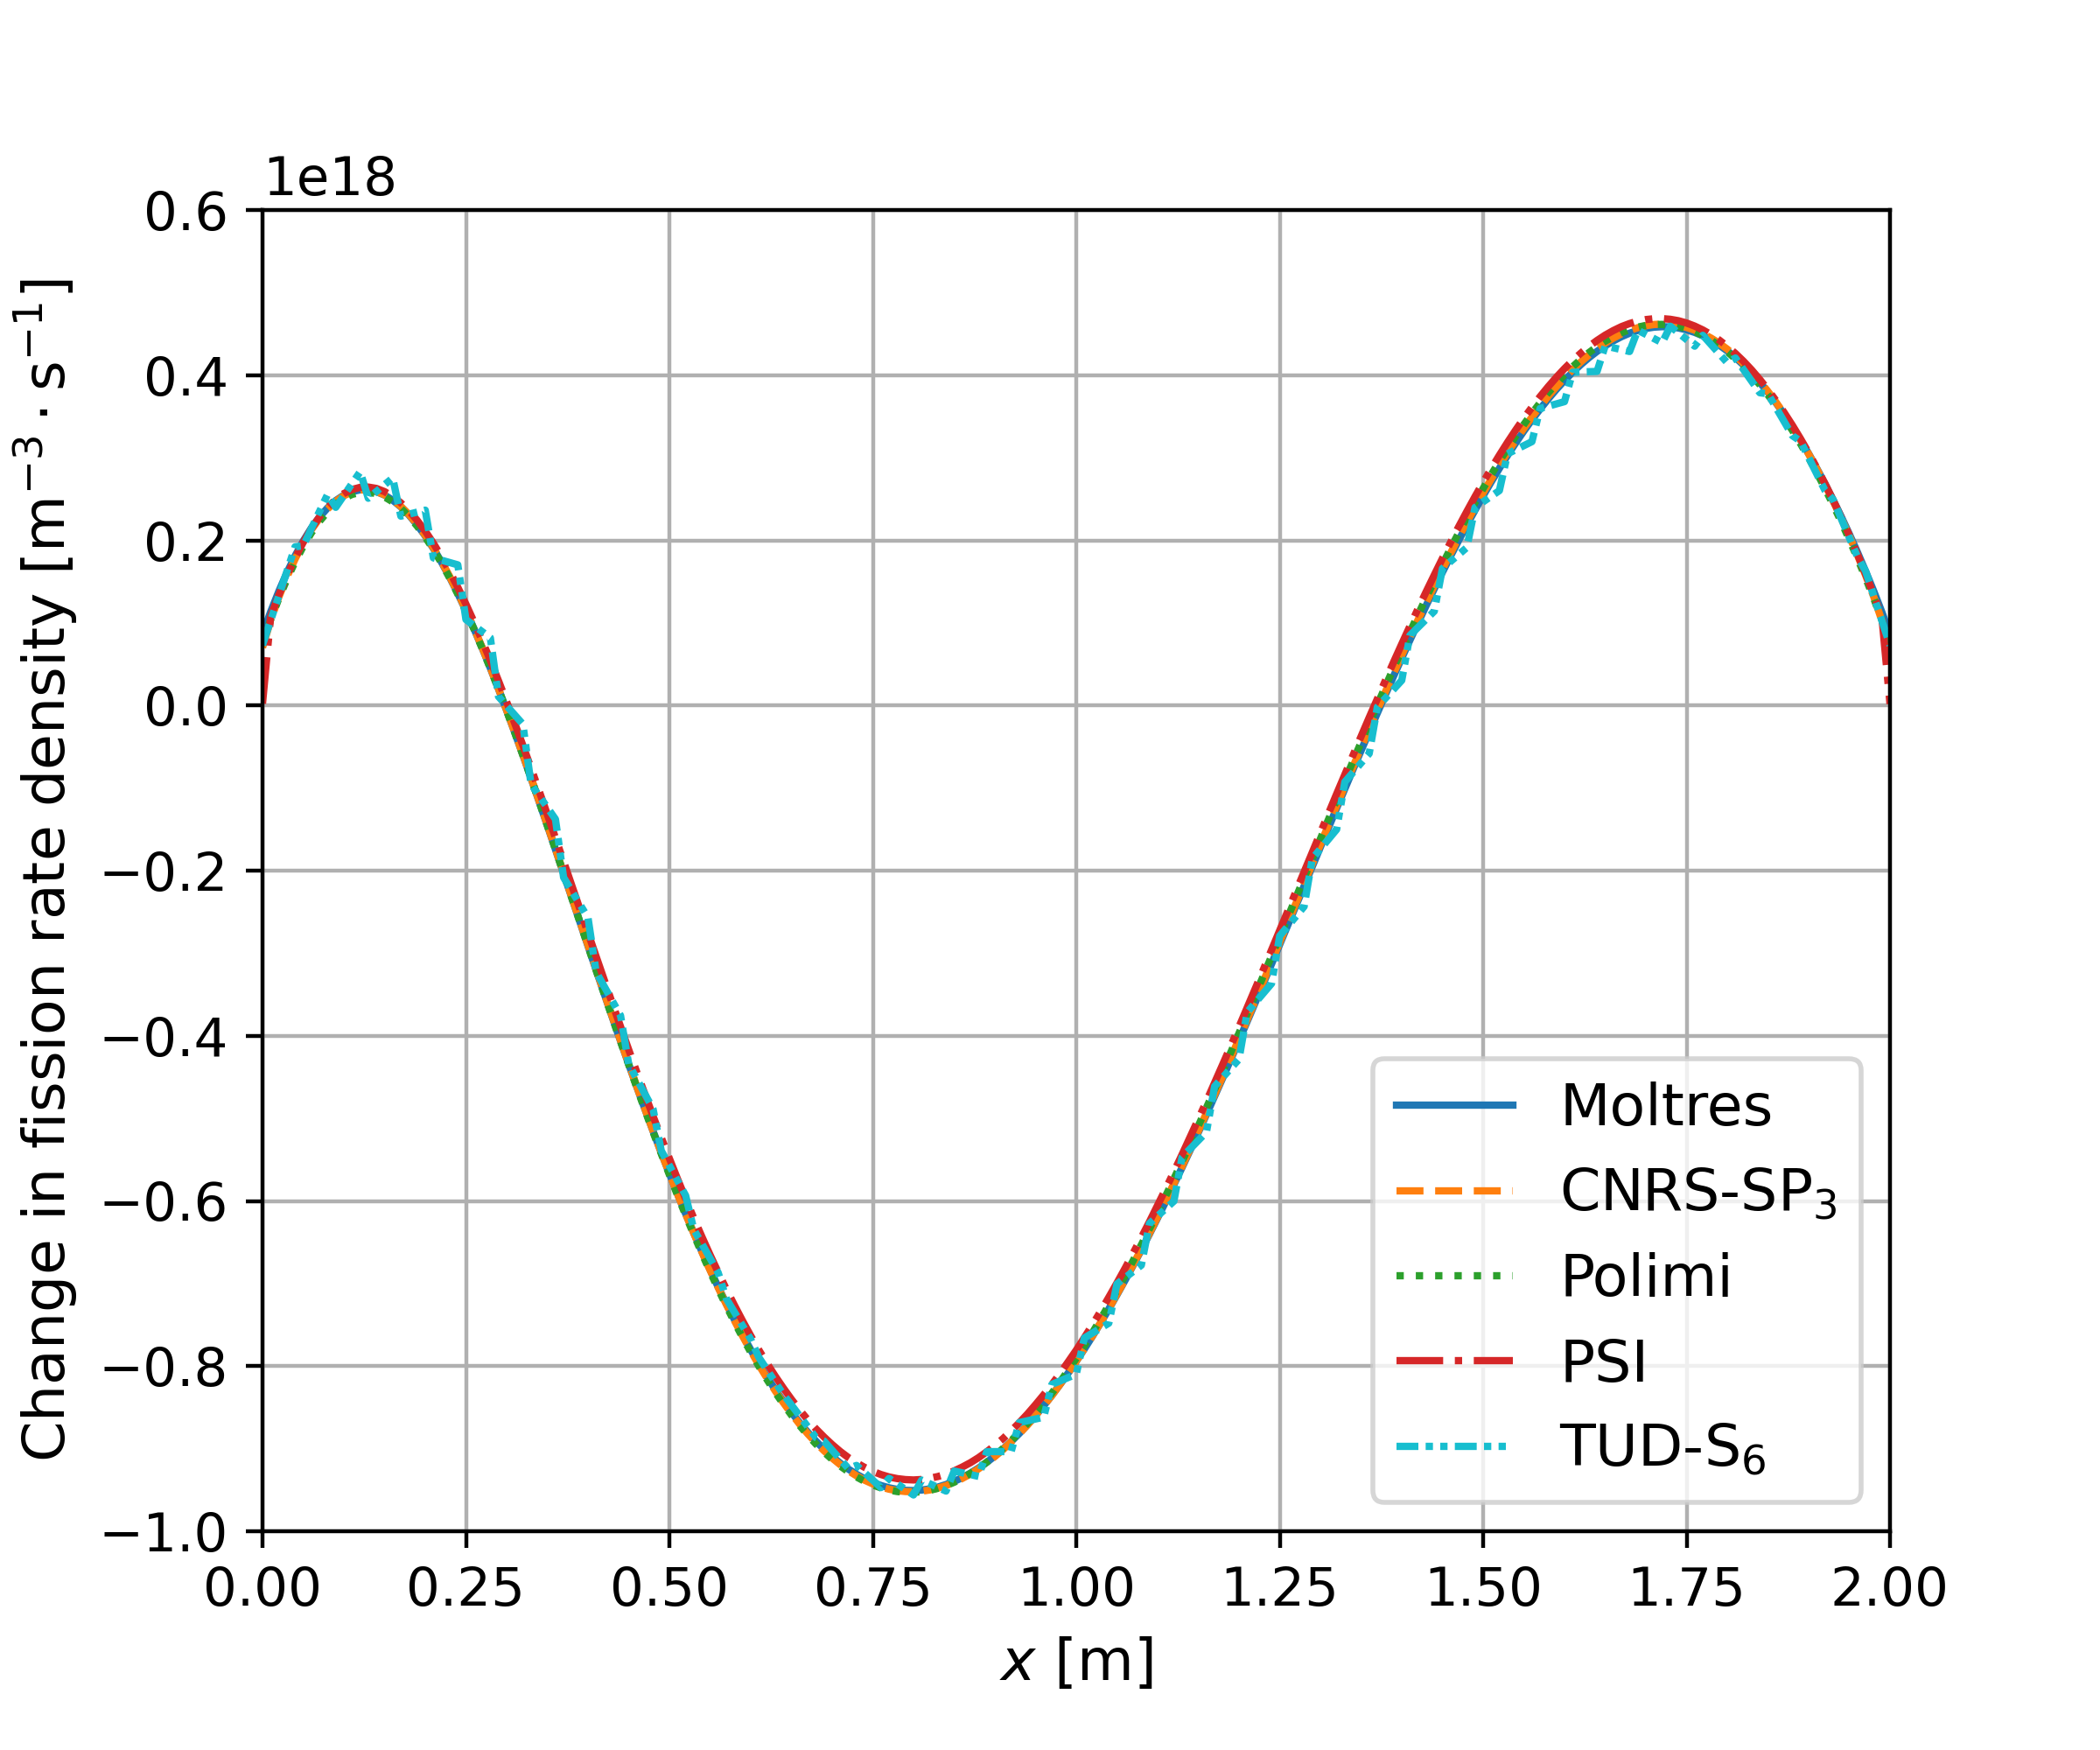
\includegraphics[width=.8\columnwidth]{1-2-fiss-plot}
	\caption{Step 1.2 - Temperature distribution and change in fission rate
	density along AA'.}
	\label{fig:1.2}
\end{figure*}

\subsubsection{Step 1.3: Buoyancy}

Moltres performs reasonably well in Step 1.3, with smaller
discrepancies in most of the velocity components and temperature distribution
than the benchmark average. Moltres bucks the trend for discrepancies
in the delayed neutron source as the discrepancy along AA' is
noticeably worse than the benchmark average, but Moltres performs relatively
better along BB'. In Table \ref{table:rho}, we observe once again that the
change in $\rho$ in Moltres falls within the range of benchmark values.
%
\begin{figure*}[h!]
	\centering
	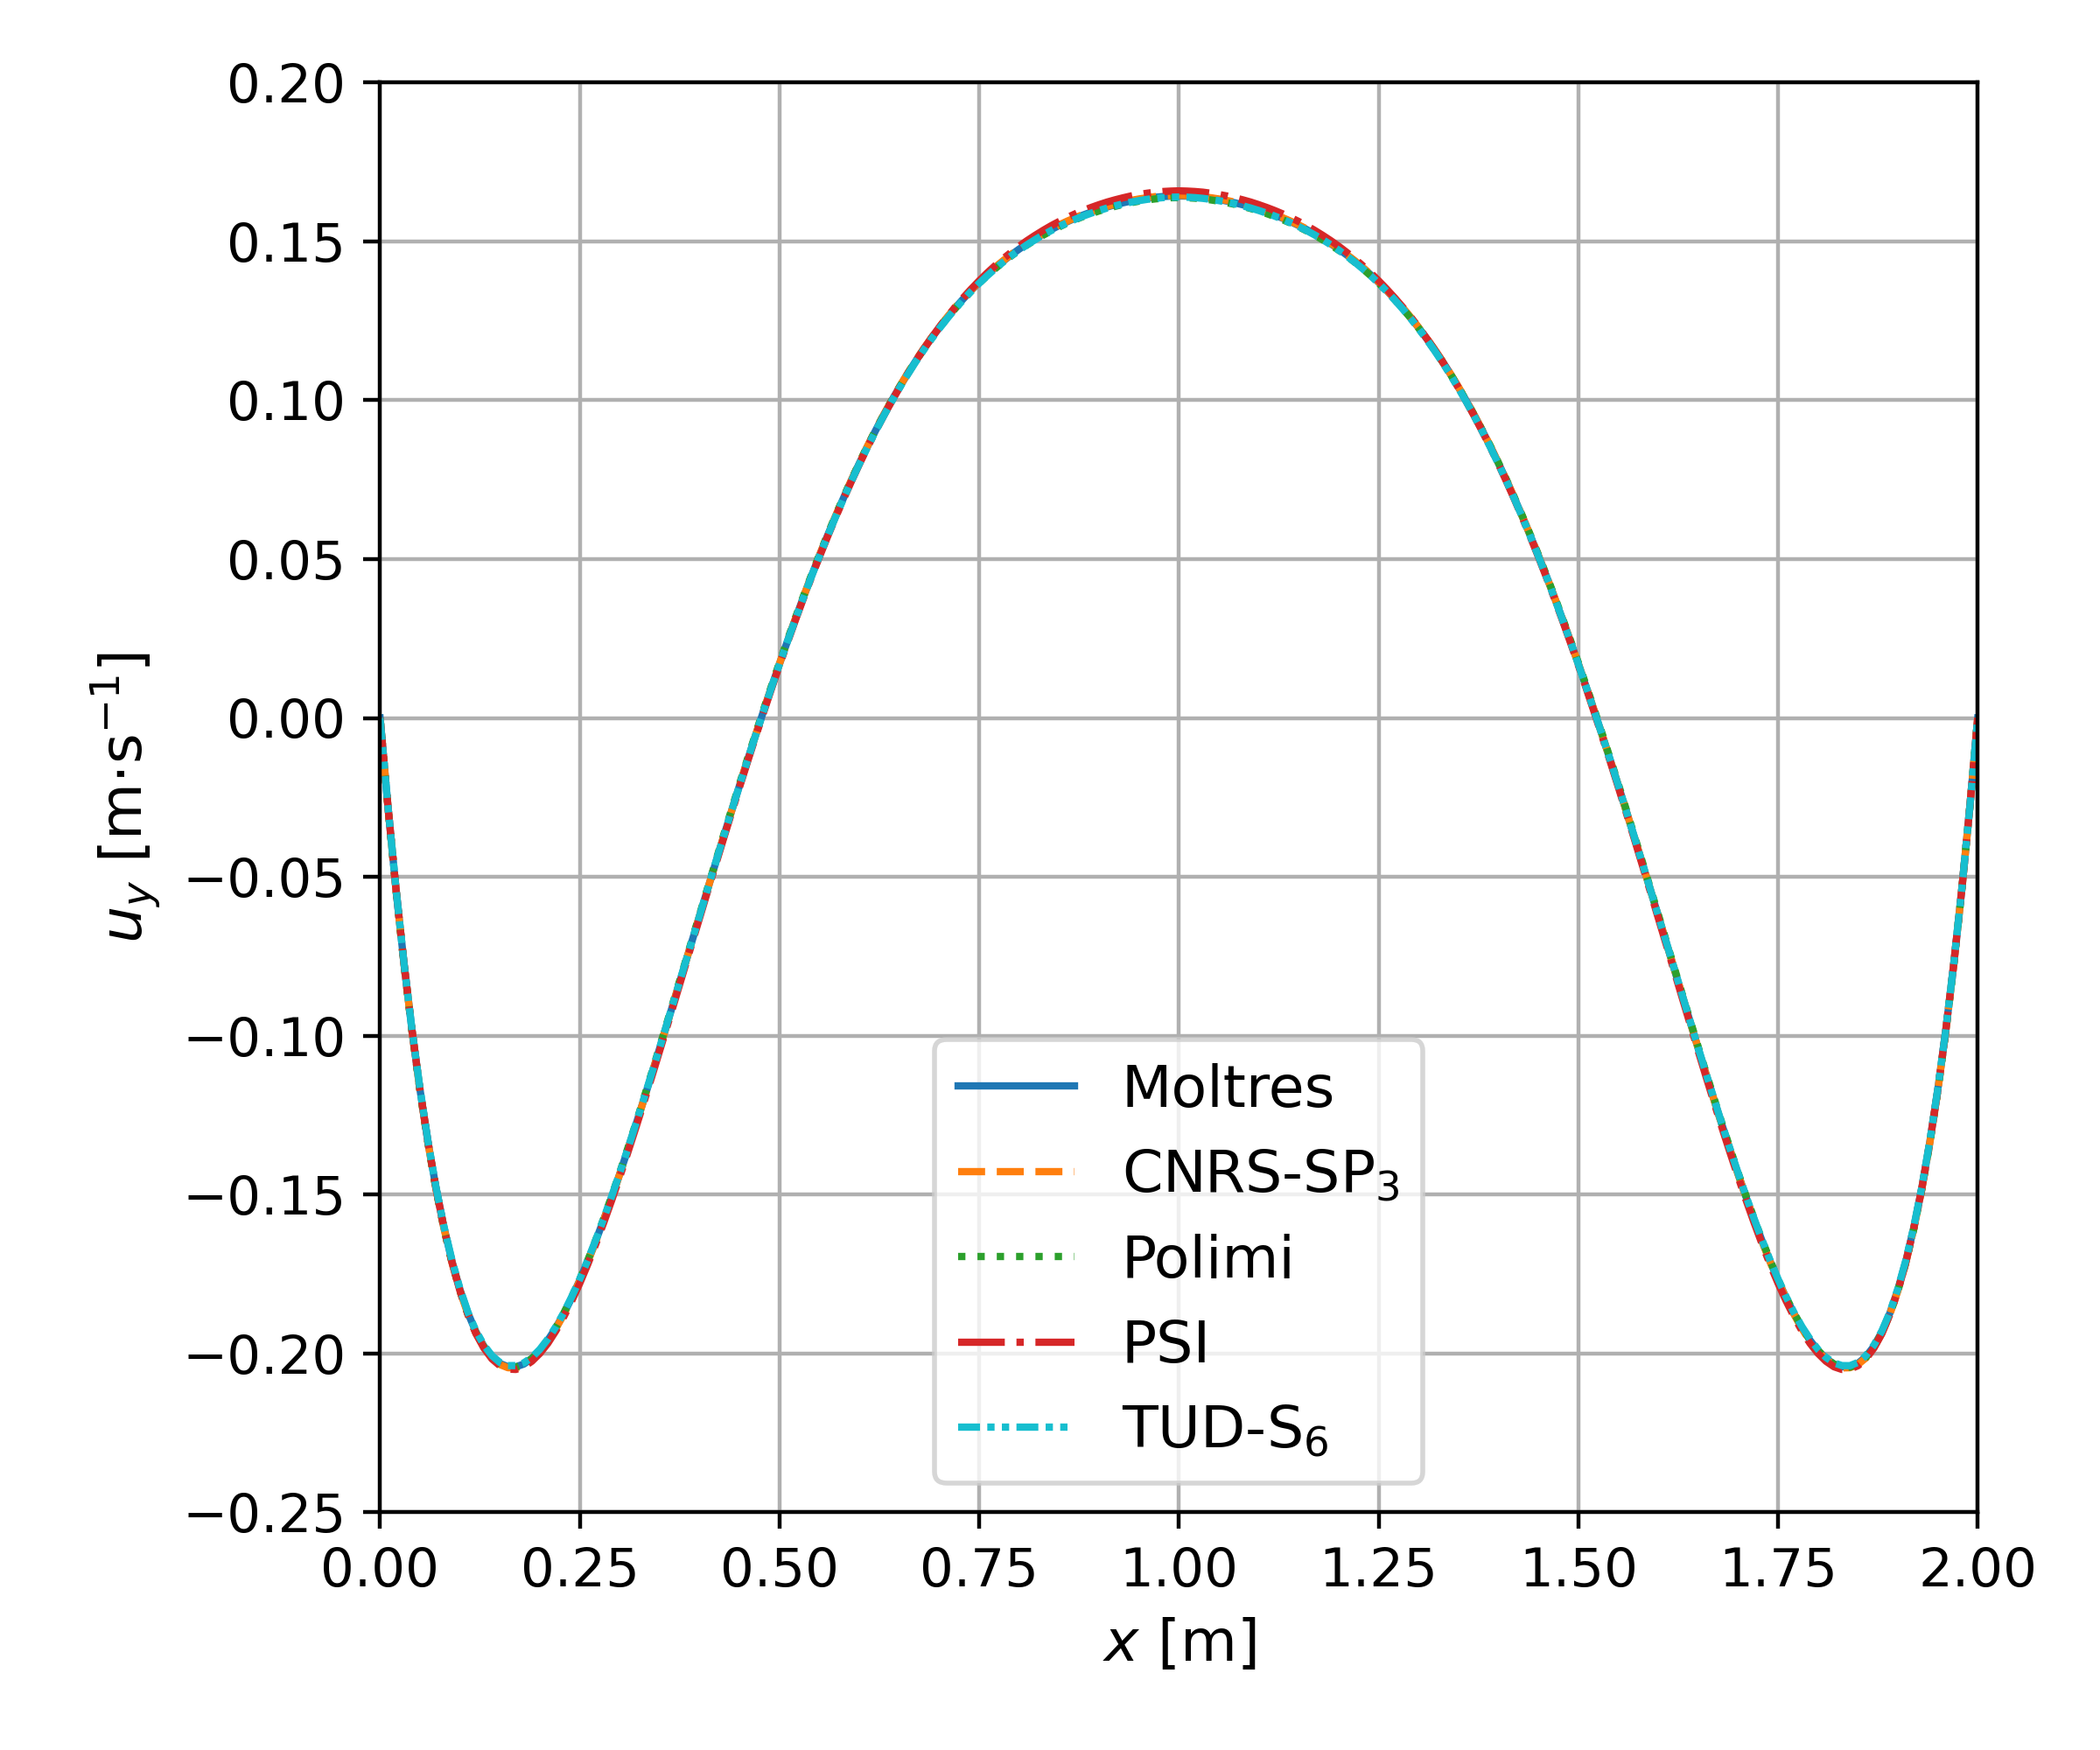
\includegraphics[width=.8\columnwidth]{1-3-vel-plot}
	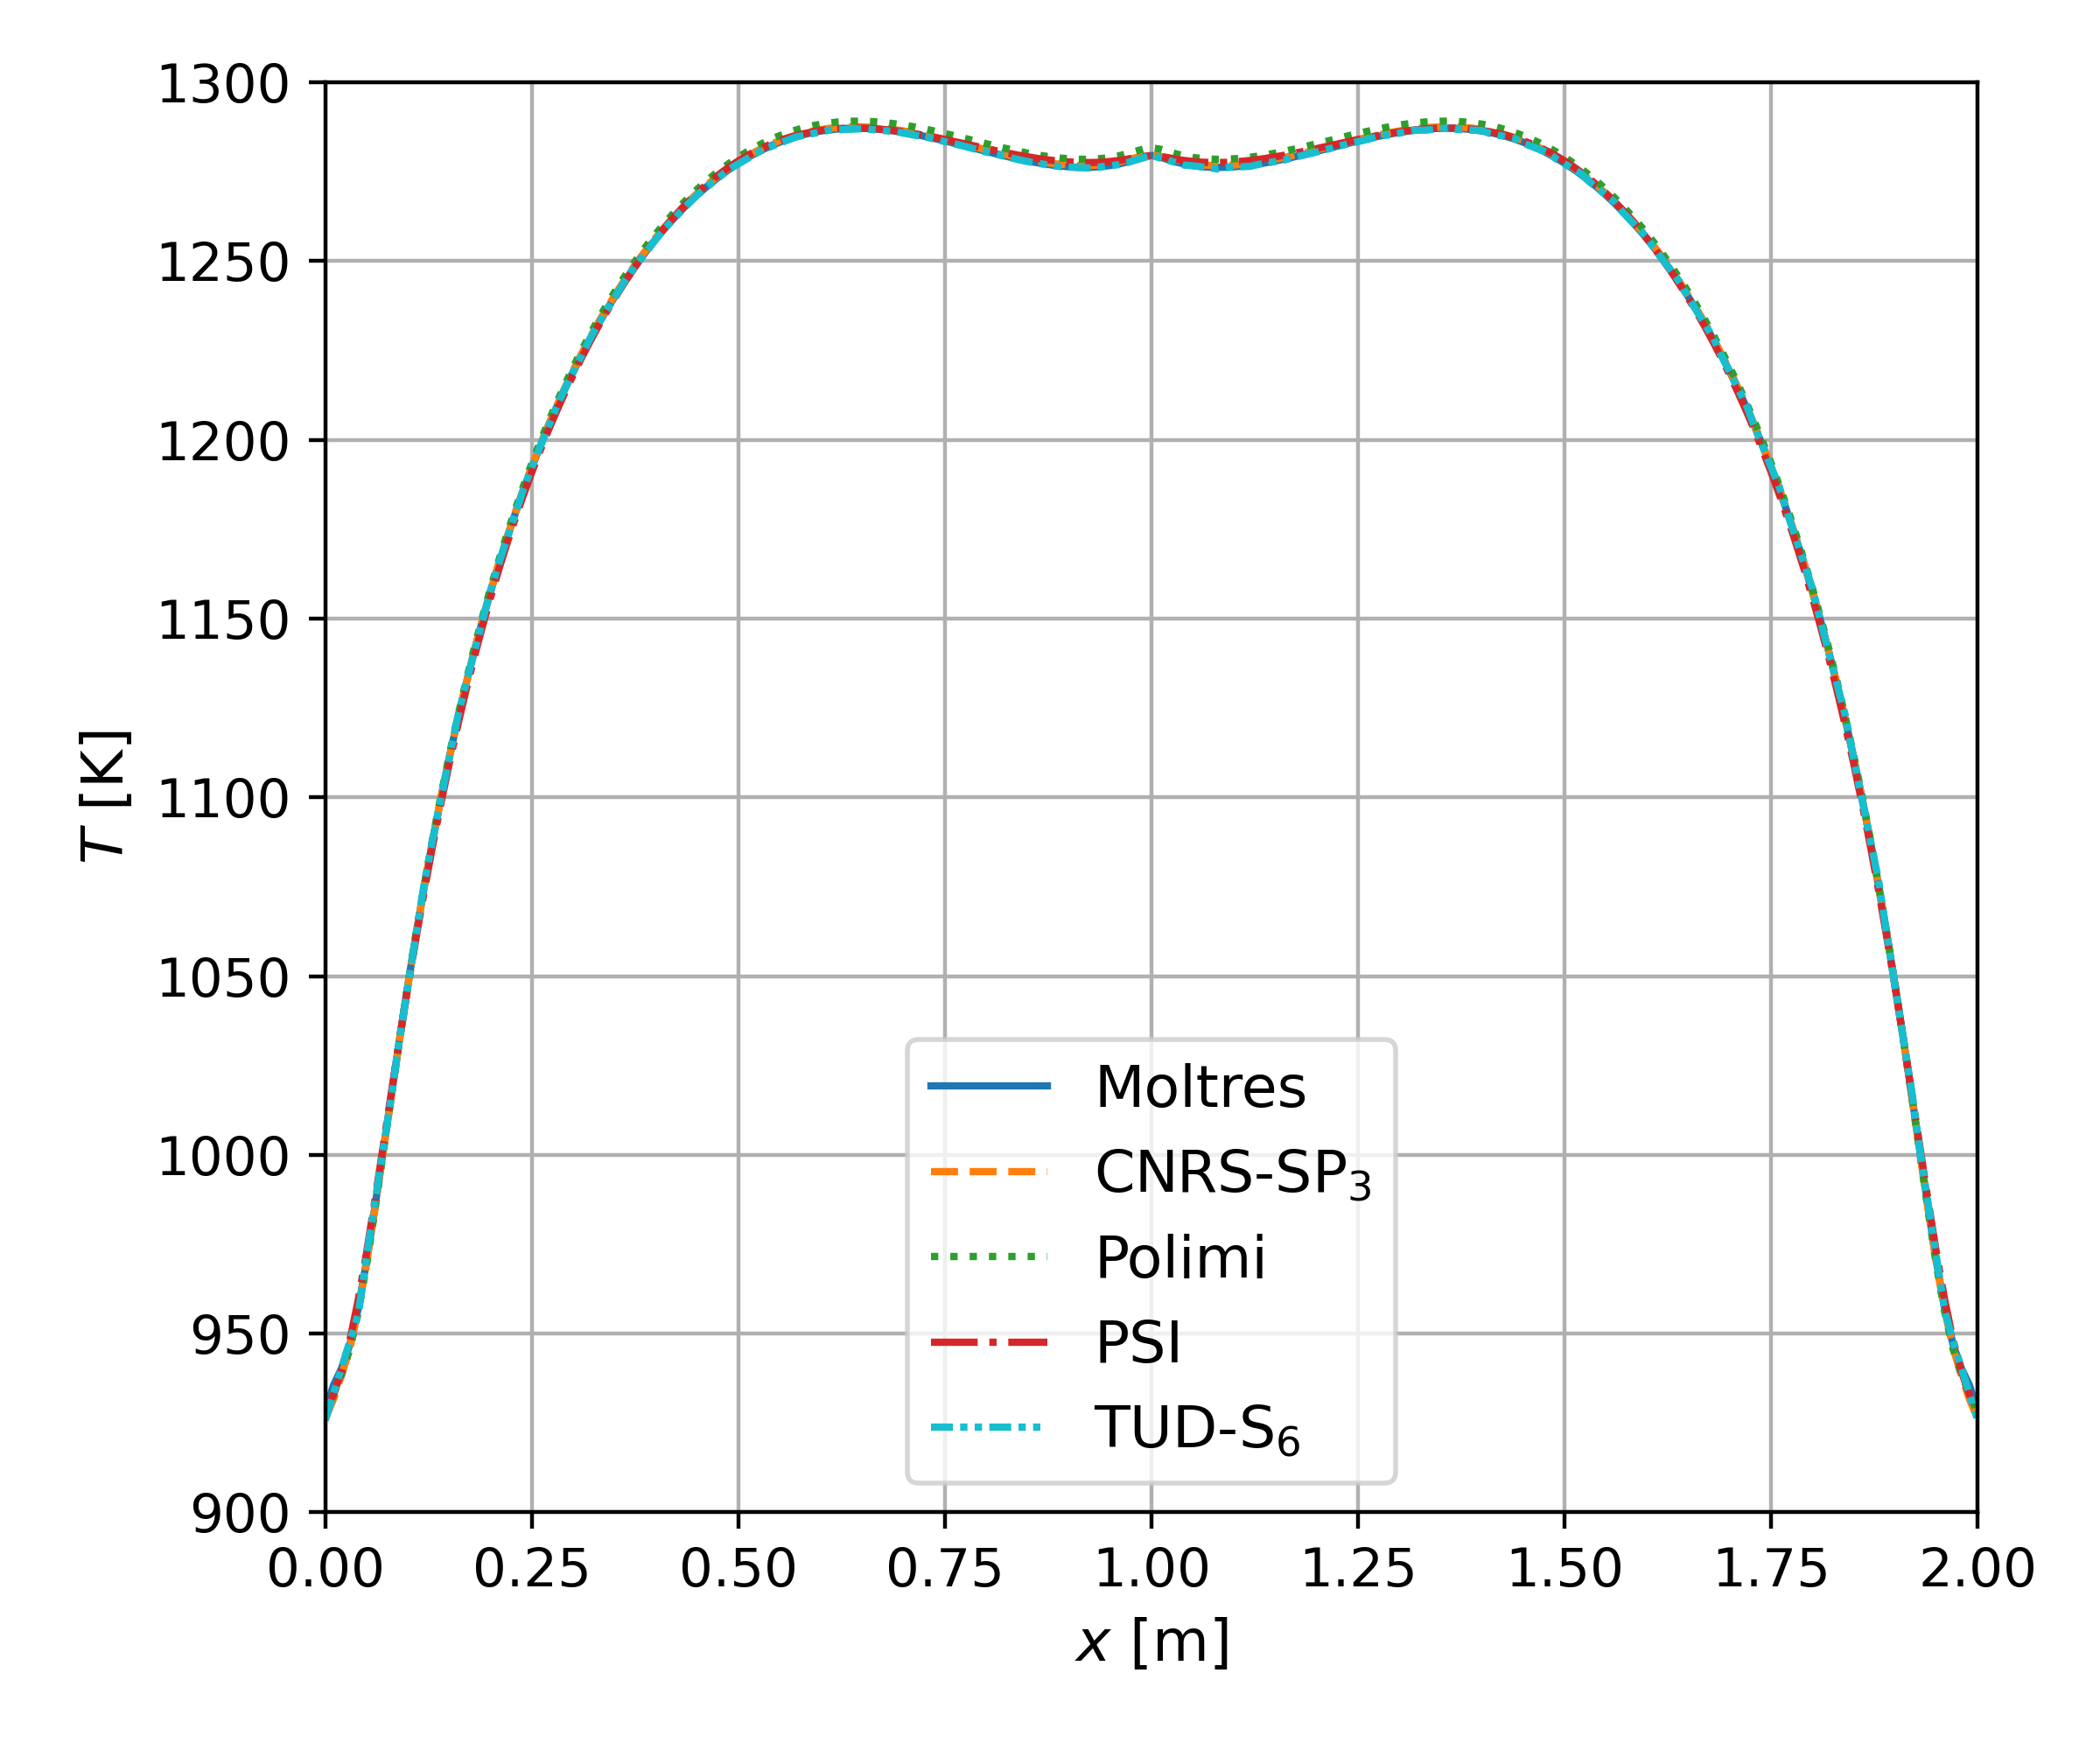
\includegraphics[width=.8\columnwidth]{1-3-temp-plot}
	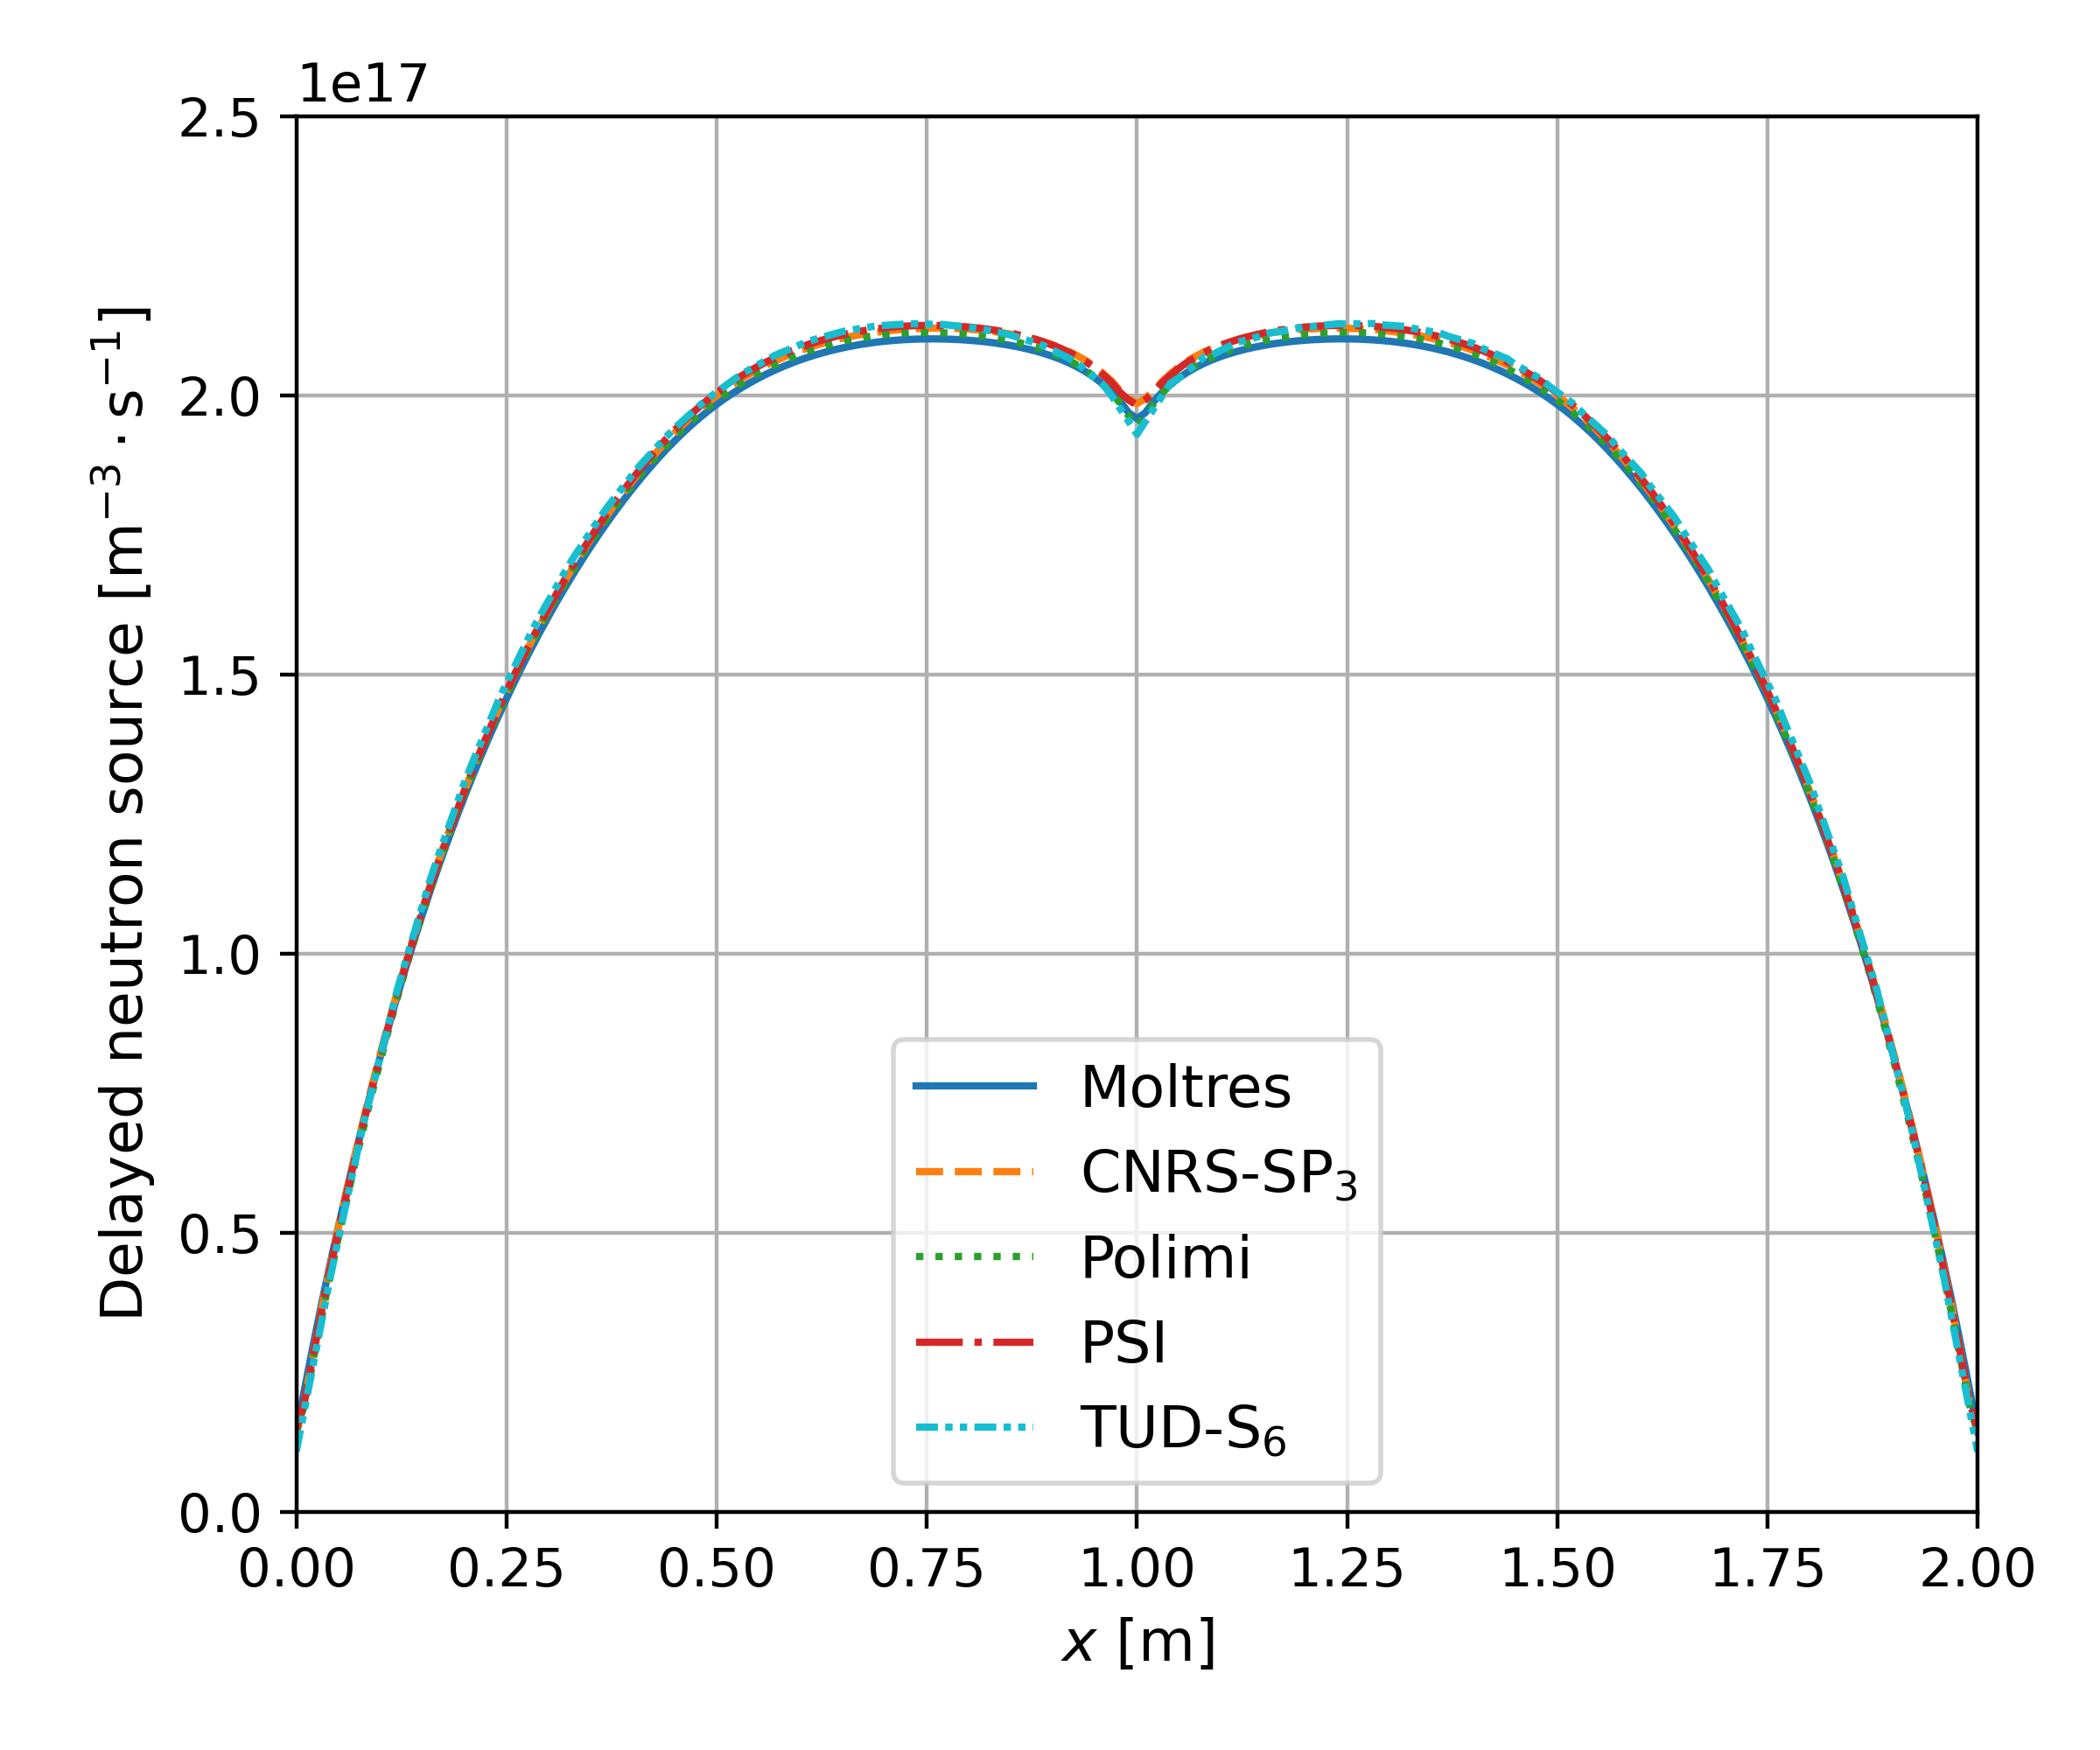
\includegraphics[width=.8\columnwidth]{1-3-dnp-plot}
	\caption{Step 1.3 - Vertical velocity component, temperature distribution,
	and delayed neutron source along AA'.}
	\label{fig:1.3}
\end{figure*}

\subsubsection{Step 1.4: Full coupling}

Table \ref{table:full} shows the change in $\rho$ under the various $U_{lid}$
and $P$ values. We refer readers to Tiberga et al.'s paper
\citep{tiberga_results_2020} for the benchmark's corresponding values.
The results from Moltres all fall within the range of benchmark values for all
cases. Furthermore, the $\Delta\rho$ values are all within 1.1 pcm of the
corresponding values from the TUD-S$_2$ model in the benchmark paper. Given
that the $S_2$ discrete ordinates method is qualitatively similar to the
multigroup neutron diffusion method, this shows that Moltres is
consistent to the benchmark within the limitations brought about by the neutron
diffusion method.

\begin{table}[htbp!]
	\caption{Reactivity change in Step 1.4, relative to Step 0.2 under various
	$U_{lid}$ and $P$ values.}
	\centering
	\footnotesize
	\setlength\tabcolsep{1.5pt}
	\begin{tabular}{c c c c c c}
		\toprule
		& \multicolumn{5}{c}{$\rho - \rho_{s0.2}$ [pcm]} \\
		\midrule
		{\backslashbox{$U_{lid}$ [m$\cdot$s$^{-1}$]}{$P$ [GW]}} & 0.2 & 0.4 & 0.6 & 0.8 & 1.0 \\
		\midrule
		0.0 & -263.7 & -498.3 & -730.9 & -966.7 & -1207.7 \\
		0.1 & -265.9 & -498.7 & -730.6 & -966.0 & -1206.7 \\
		0.2 & -268.1 & -498.8 & -729.4 & -963.7 & -1203.6 \\
		0.3 & -269.9 & -498.5 & -727.8 & -960.8 & -1199.5 \\
		0.4 & -271.9 & -498.5 & -726.5 & -958.3 & -1195.7 \\
		0.5 & -274.2 & -498.7 & -725.6 & -956.4 & -1192.7 \\
		\bottomrule
	\end{tabular}
	\label{table:full}
\end{table}

\subsection{Phase 2 results \& discussion}

\subsubsection{Step 2.1: Forced convection transient}
%
\begin{figure*}[h!]
	\centering
	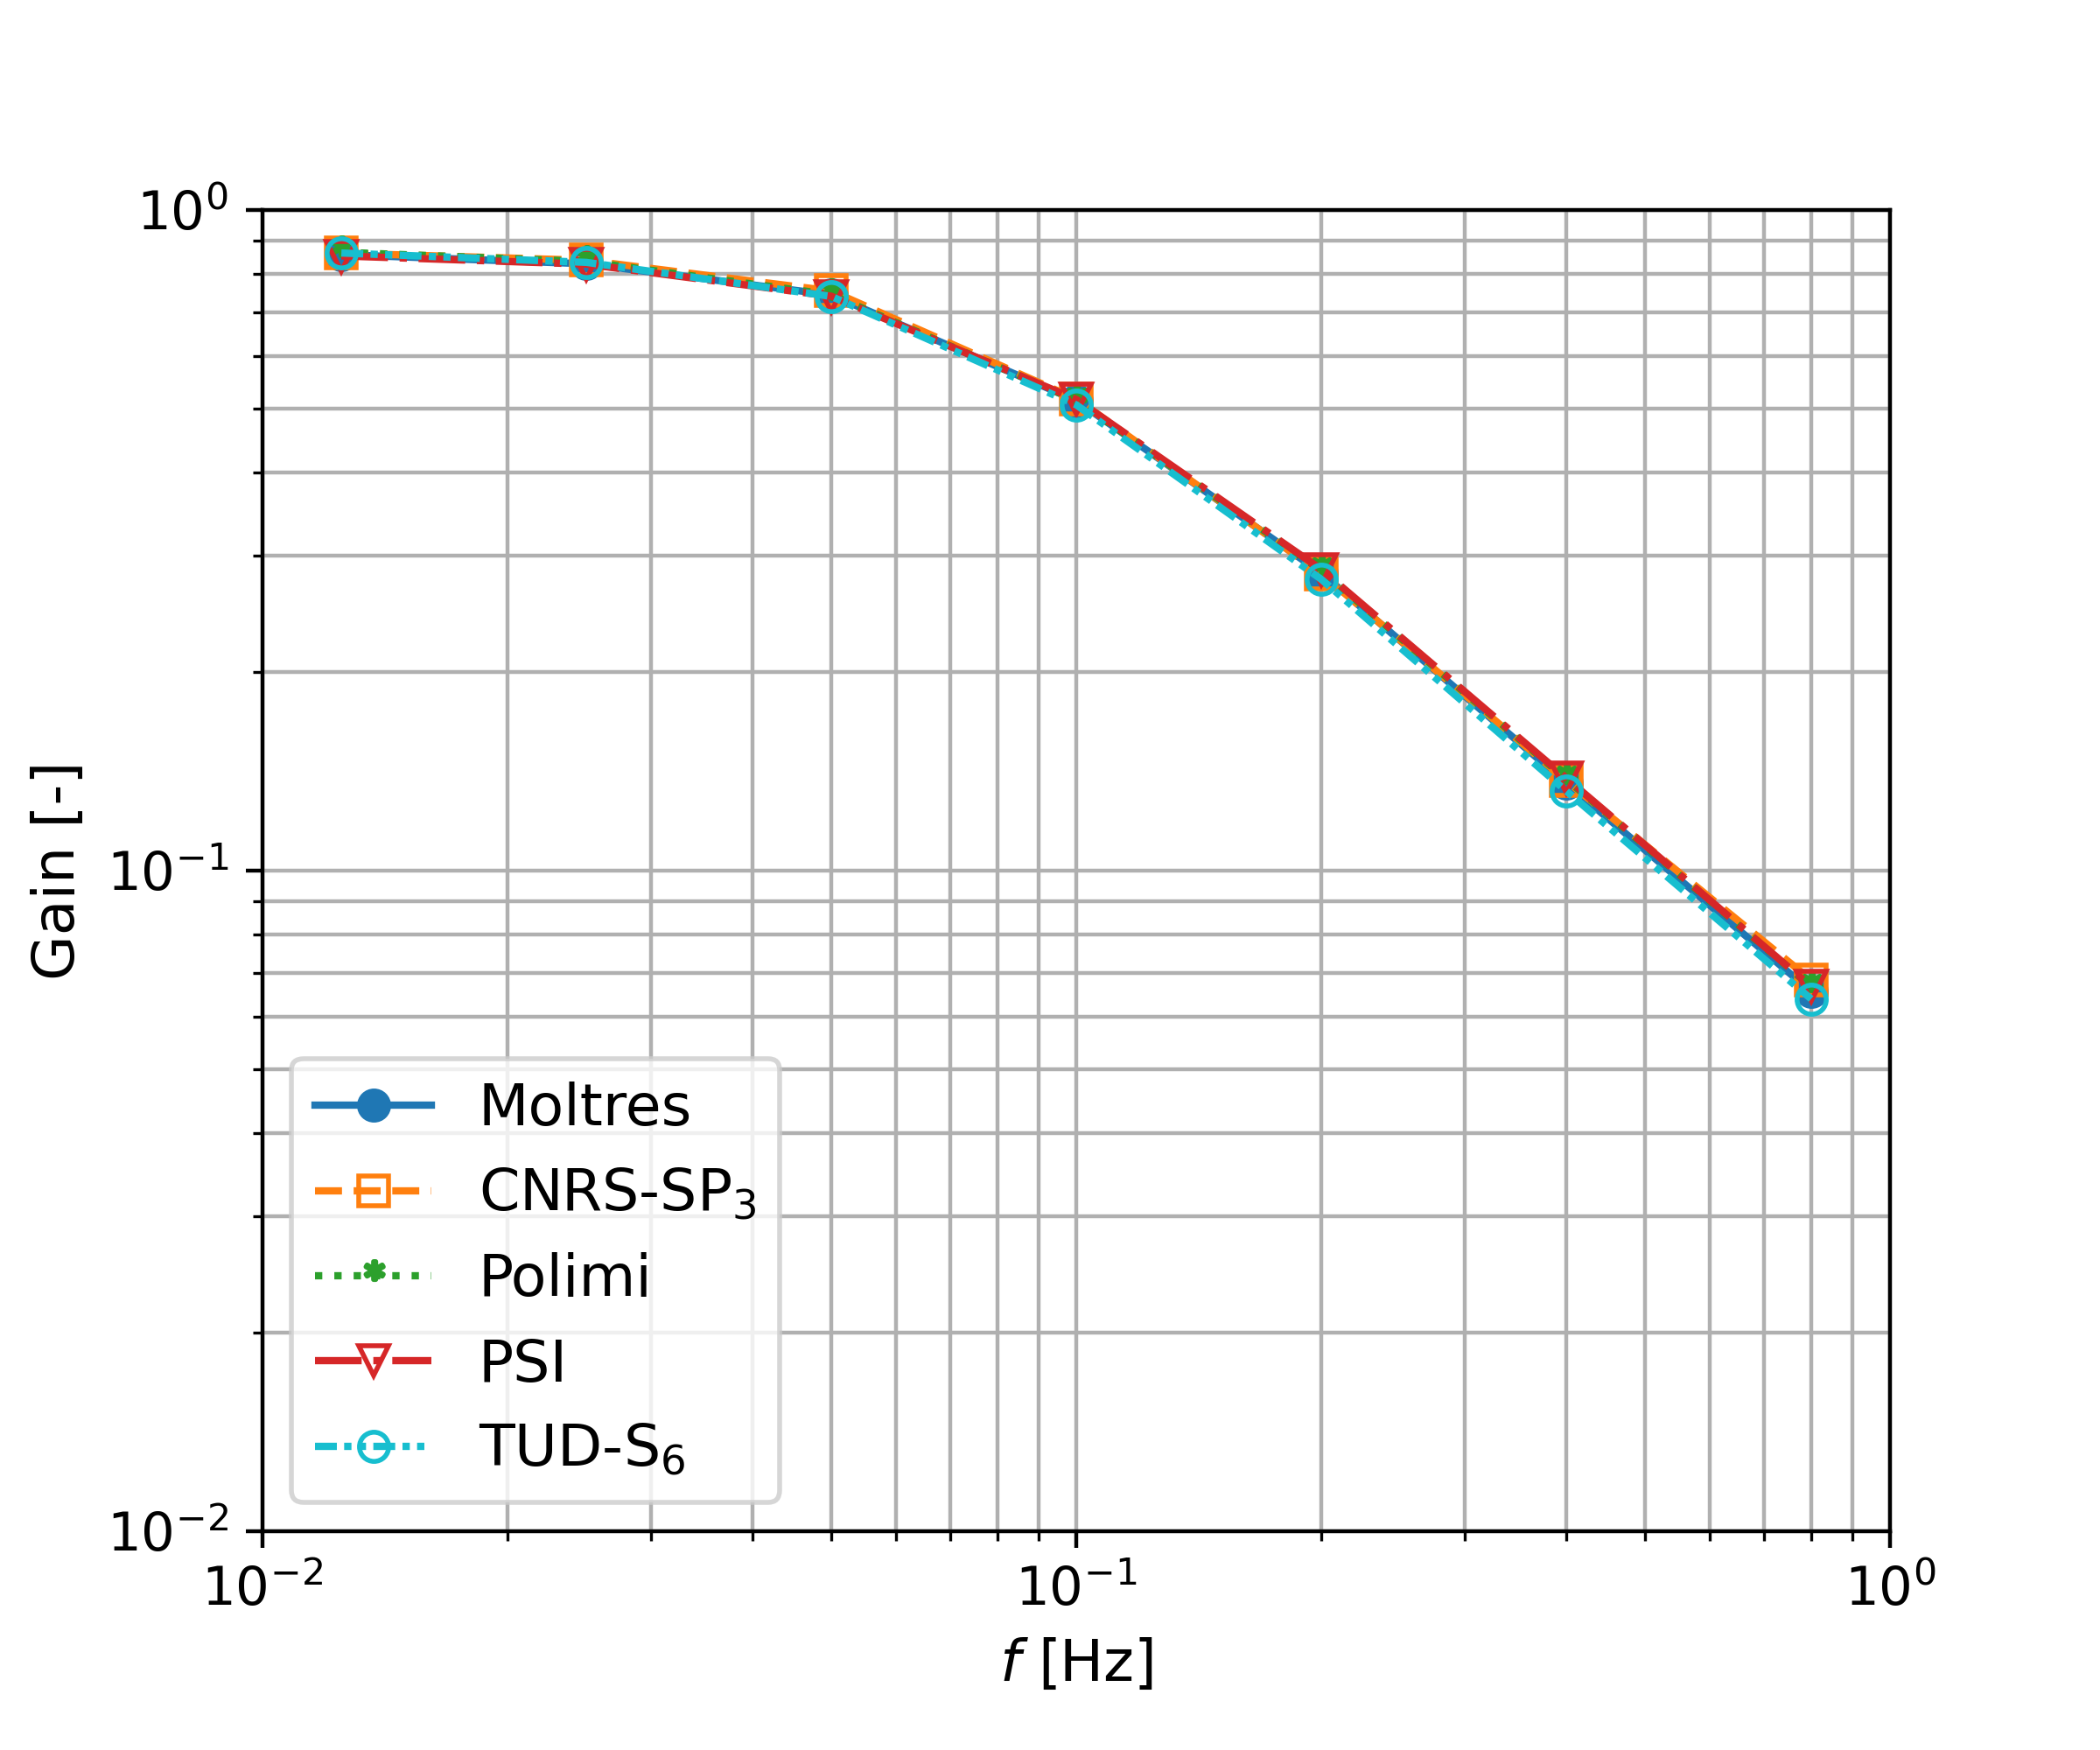
\includegraphics[width=.8\columnwidth]{2-1-gain-plot}
	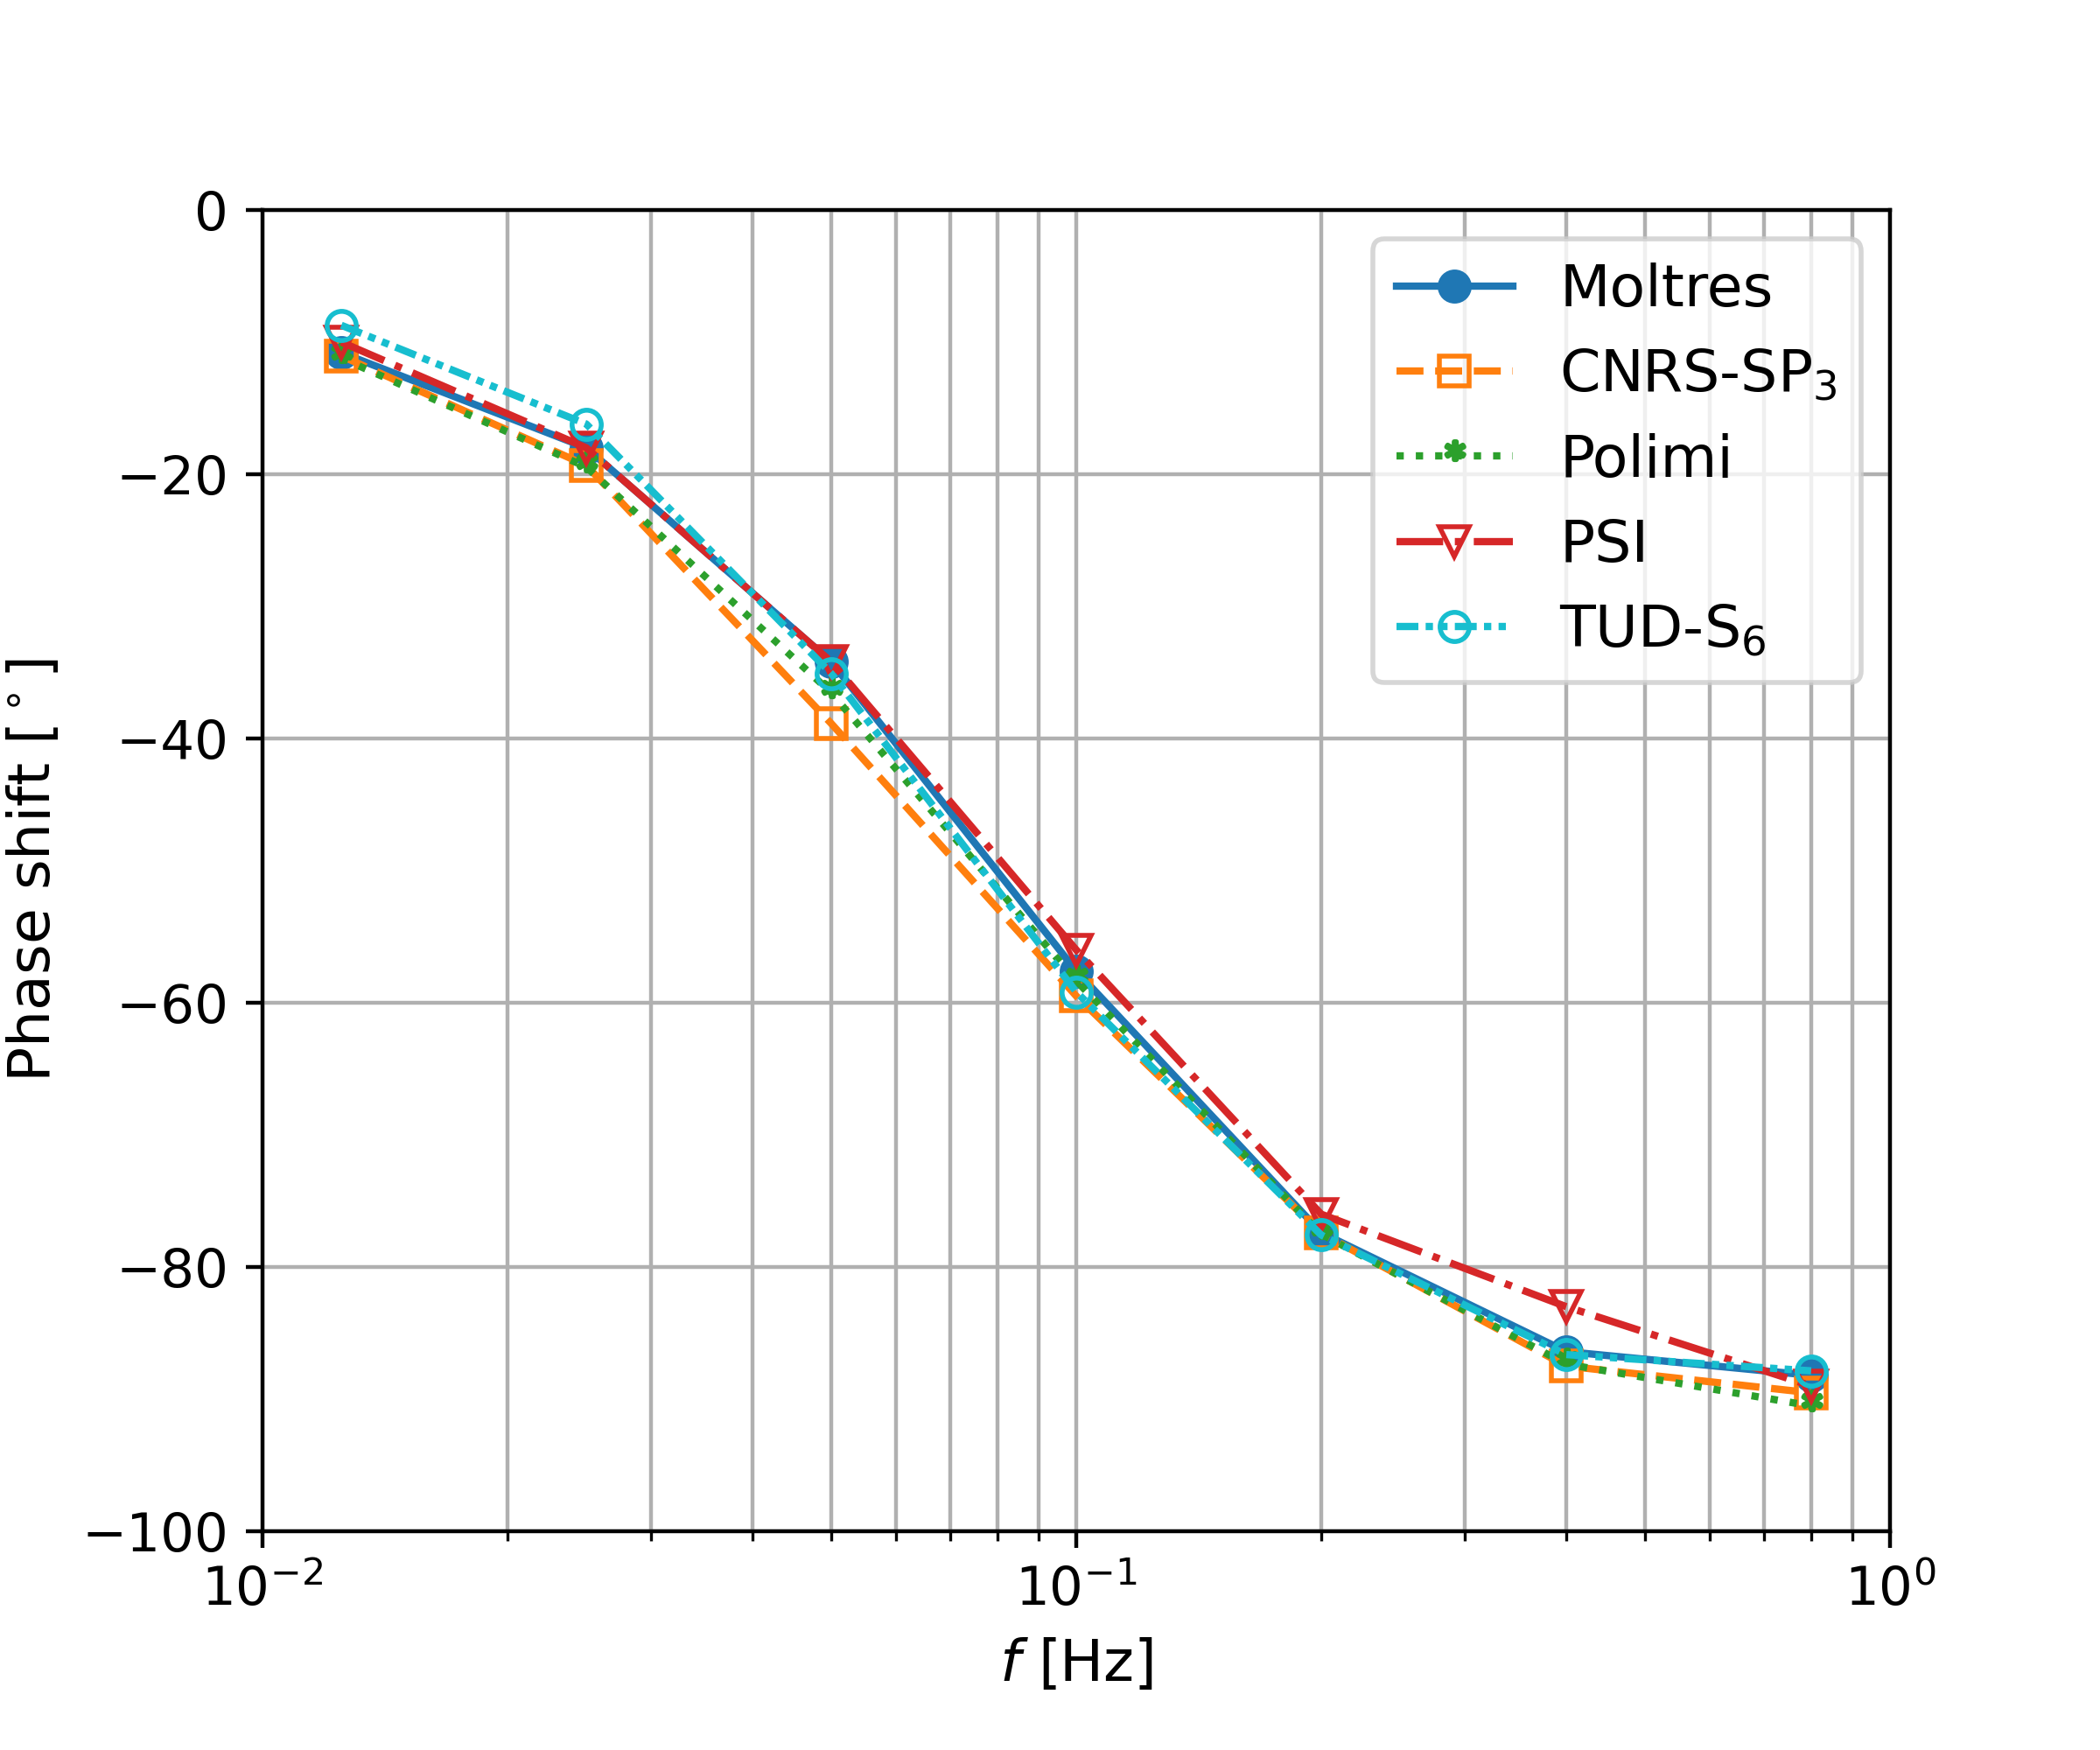
\includegraphics[width=.8\columnwidth]{2-1-phase-plot}
	\caption{Step 2.1 - Bode gain and phase plots of the frequency response of
	the fully coupled system.}
	\label{fig:2.1}
\end{figure*}

